\documentclass[11pt,letterpaper]{article}
\input{headings}
\newcommand \recipeName {Chicken with A Lemon}
\newcommand \fileName {ChickenWithALemon}
\chead{\recipeName}

\begin{document}
\input{title}

``Chicken with Two Lemons'' is a recipe that made Marcella Hazan famous when it was published by the \href{https://cooking.nytimes.com/recipes/1015182-marcella-hazans-roast-chicken-with-lemons}{\it New York Times}. It is a very good recipe. But, I made a few changes to it, incorporating the steps of removing the wishbones (thanks to Julia Child) and removing the kidneys from inside the chicken (thanks to Jacques Pepin), and  brining and air drying the chicken (thanks to America's Test Kitchen) to ensure that it results in a moist breast meet. The sugar in the brining also encourages brining. I also found out that warming the roasting pan in the oven and spraying it with cooking spray is a good insurance to prevent the chicken from sticking to the pan. For sewing the chicken I use a narding needle that I purchased in a sewing shop (see picture).

 
\begin {description}

\item[Ingredients:]\ \\
\begin{itemize}
	\item 1 roasting chicken (or two smaller birds)
	\item 1/4 cup of salt
	\item 1/4 cup of sugar
	\item 1 yellow lemon
	\item black pepper
	\item cooking spray
\end{itemize}

\item[Procedure:]\ \\

\begin{enumerate}
\item {\bf Prepare the Chicken}
\begin{itemize}
\item Remove from package, wash it very well under running cold water, make sure to remove any blood from the cavity. 
\item Check for the kidneys. If they are still attached to the back bone inside the cavity, remove them by first running a small sharp knife along the edges to cut the membranes that attach the kidneys to the back bone and then scraping with your finger under running water.
\end{itemize}

\item {\bf Remove the Wish Bone}
\begin{itemize}
\item Place the chicken in the counter so that the breast opening faces you. 
\item Feel for the wish bone along the front of the breast. 
\item With a paring knife, make incisions along the wish bone, and remove the wish bone. 
\end{itemize}

\item {\bf Brine the Chicken}
\begin{itemize}
\item In a deep mixing bowl mix 1/2 cup of salt and 1/4 cup of sugar with 2 quarts of water and stir well. 
\item Submerse the chicken in the brine, put in the refrigerator and let it brine for at least 2 hours, and up to 8 hours.
\end{itemize}



\item {\bf Season the chicken, prep the Lemon and Sew the lemon inside chicken and air dry it}
\begin{itemize}
\item Sprinkle the chicken inside and out with freshly ground black pepper.
\item Wash the lemons and dry wiht a cloth.
\item With a toothpick, poke many holes into the lemon.
\item Put the lemon inside the cavity of the chicken.
\item Using a large needle (I use a narding needle) and kitchen string, sew both ends of the chicken cavity shut.
\item Place the chicken, brest-side up on a baking tray fitted with a cooling rack and place in the refrigerator to air dry it. Keep in the refrigerator for several hours.
\end{itemize}

\item{\bf Preheat the oven to 350 degrees}
\begin{itemize}
\item Put an empty roasting pan in the oven when you turn the oven on to pre-heat it. 
\end{itemize}

\item{\bf Roast the chicken}
\begin{itemize}
\item Remove the pre-heated roasting pan from the oven. 
\item Spray the hot pan, and the brest side of the chicken, with cooking spray (alternatively rub it with a thin film of cooking oil).
\item Place the chicken, breast side down, on the hot pan.
\item Roast the chicken for 30 minutes.
\end{itemize}

\item{\bf Turn the chicken}
\begin{itemize}
\item Remove the chicken from the oven.
\item Using a flat spatula and oven mittens, carefully turn the chicken on its back side and return to the oven.
\item Roast for another 20 minutes.
\end{itemize}

\item{\bf Finish roasting the chicken}
\begin{itemize}
\item Increase the oven temperature to 400 degrees.
\item Roast the chicken for another 10 or 20 minutes.
\item The chicken is done when the breast registers 150 F and the thighs 160 F on an instant read thermometer.
\item Remove from the oven and place it on a platter and let it rest for  five minutes before carving.
\end{itemize}
\end{enumerate}
\end{description}

\begin{table}
\begin{tabular}{cccc}
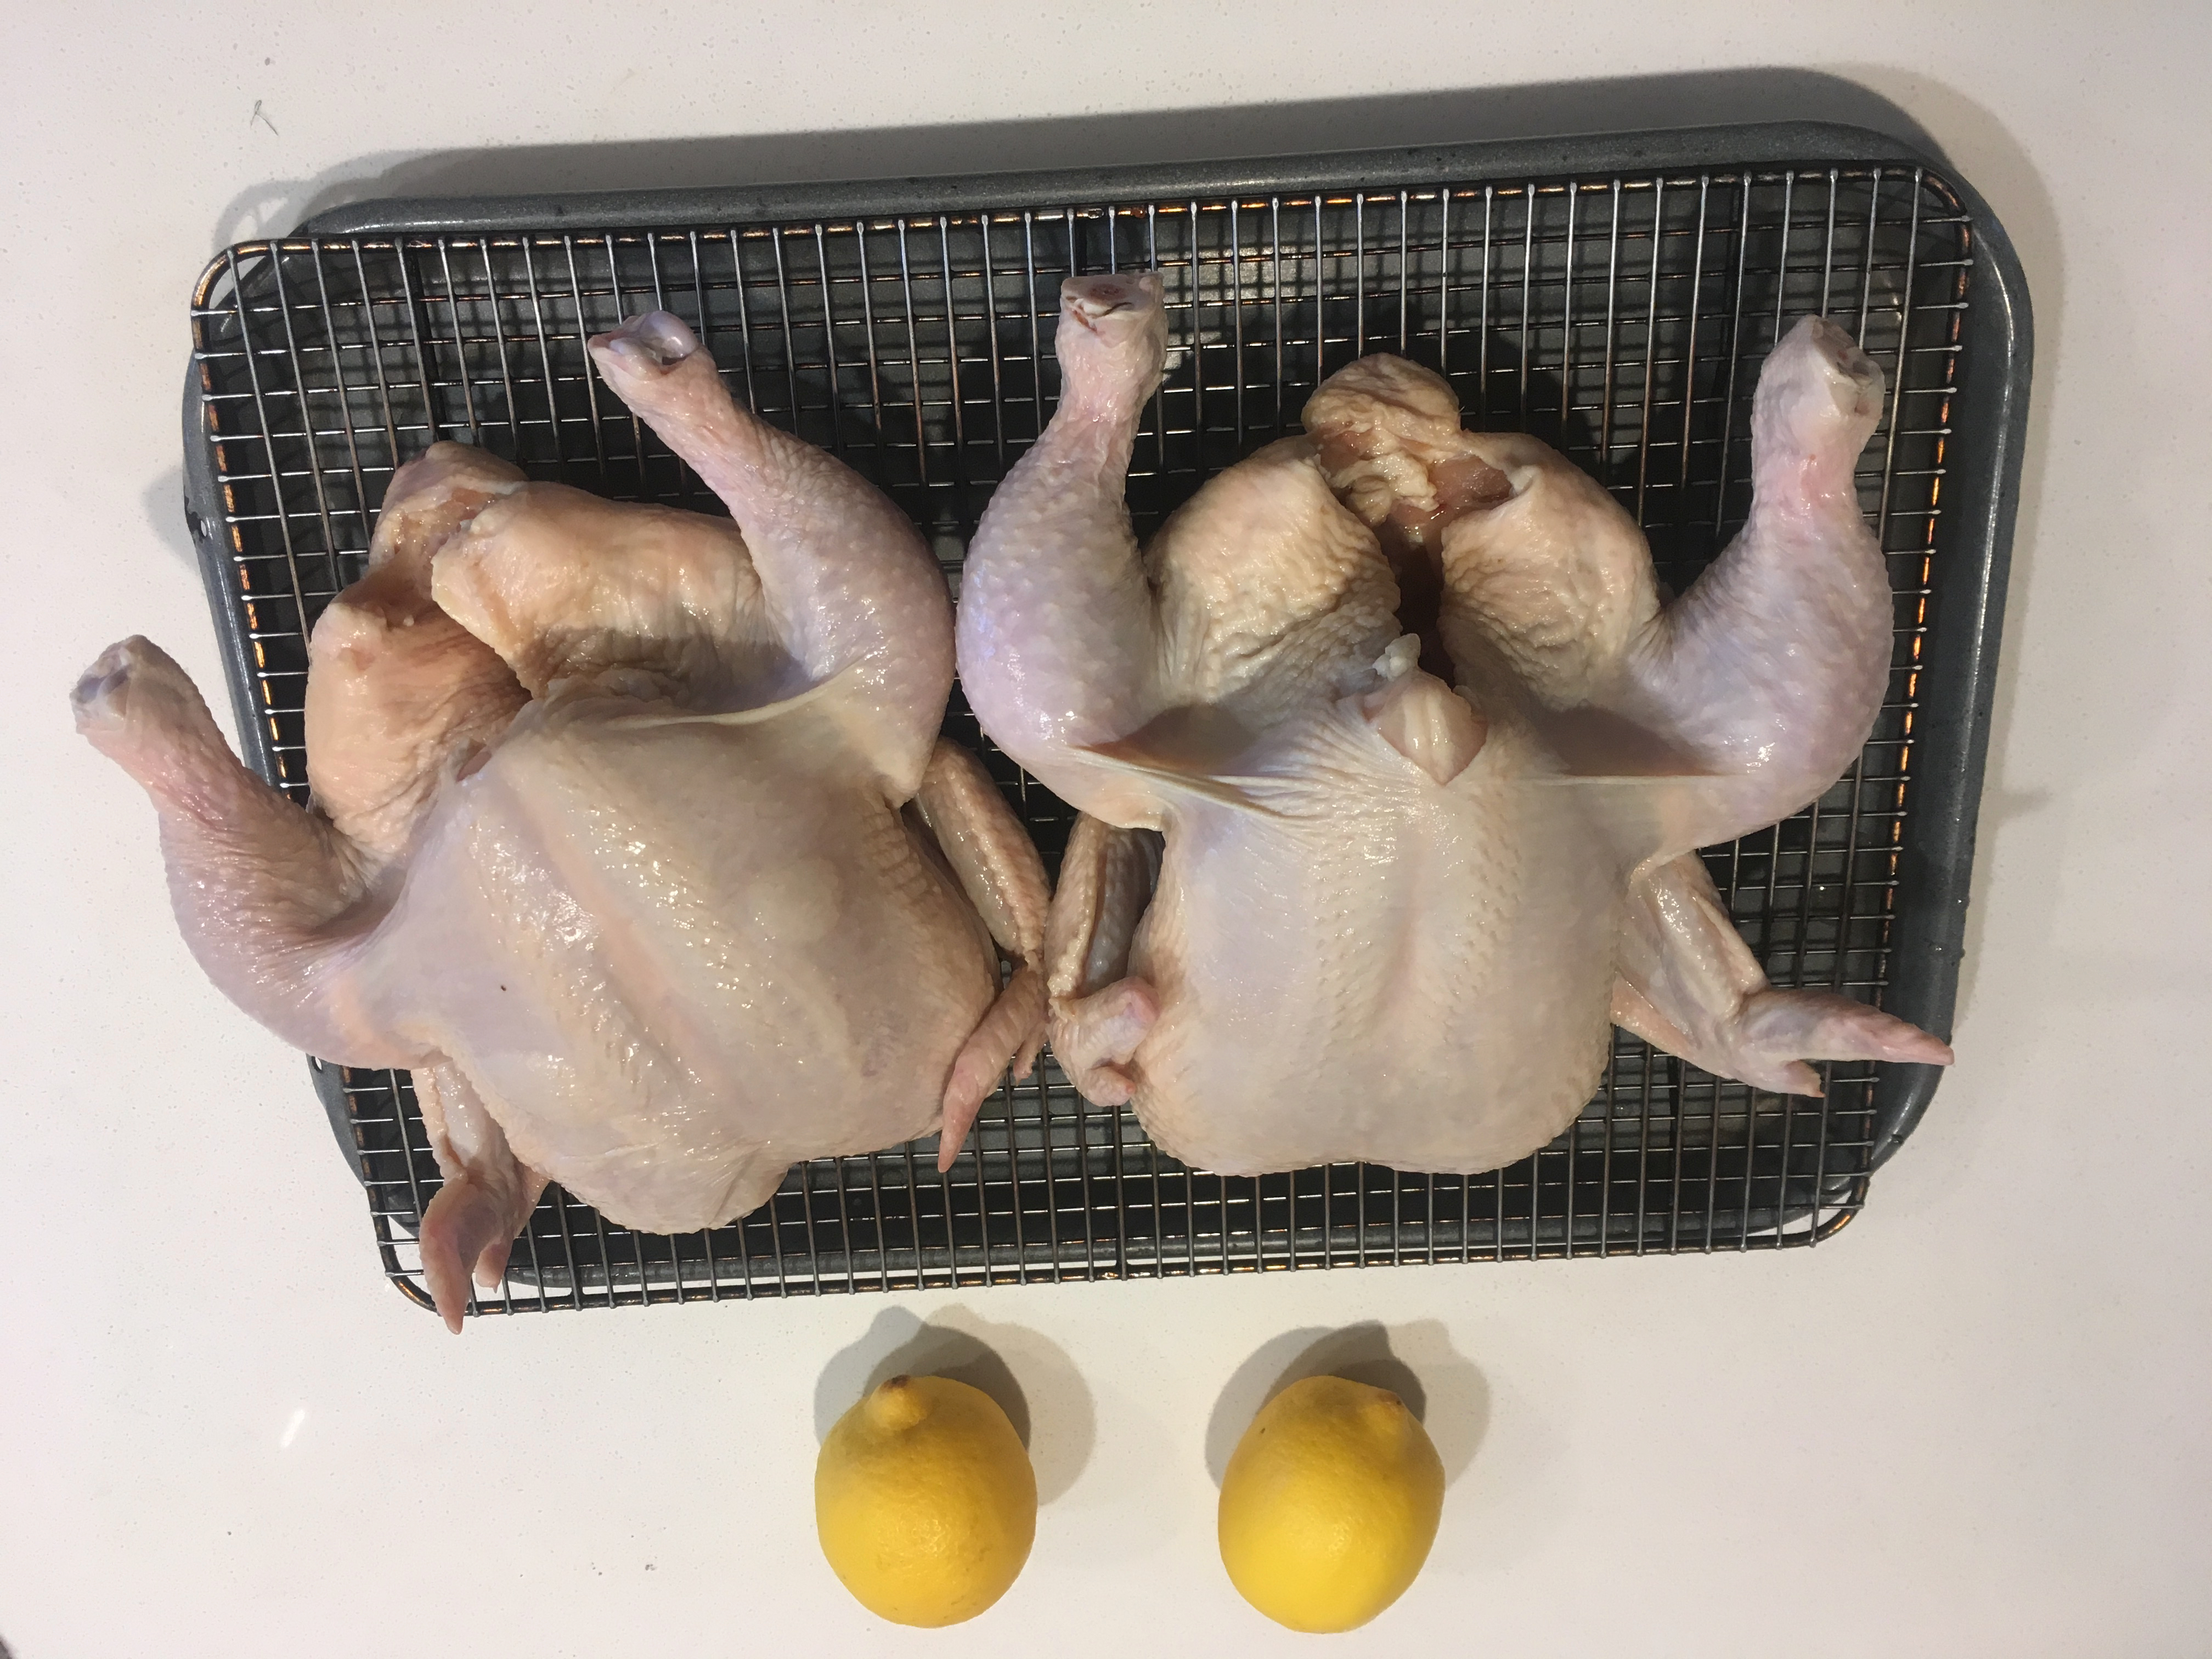
\includegraphics[width=0.25\textwidth]{\imageDir/\fileName/IMG_3197.jpg} &
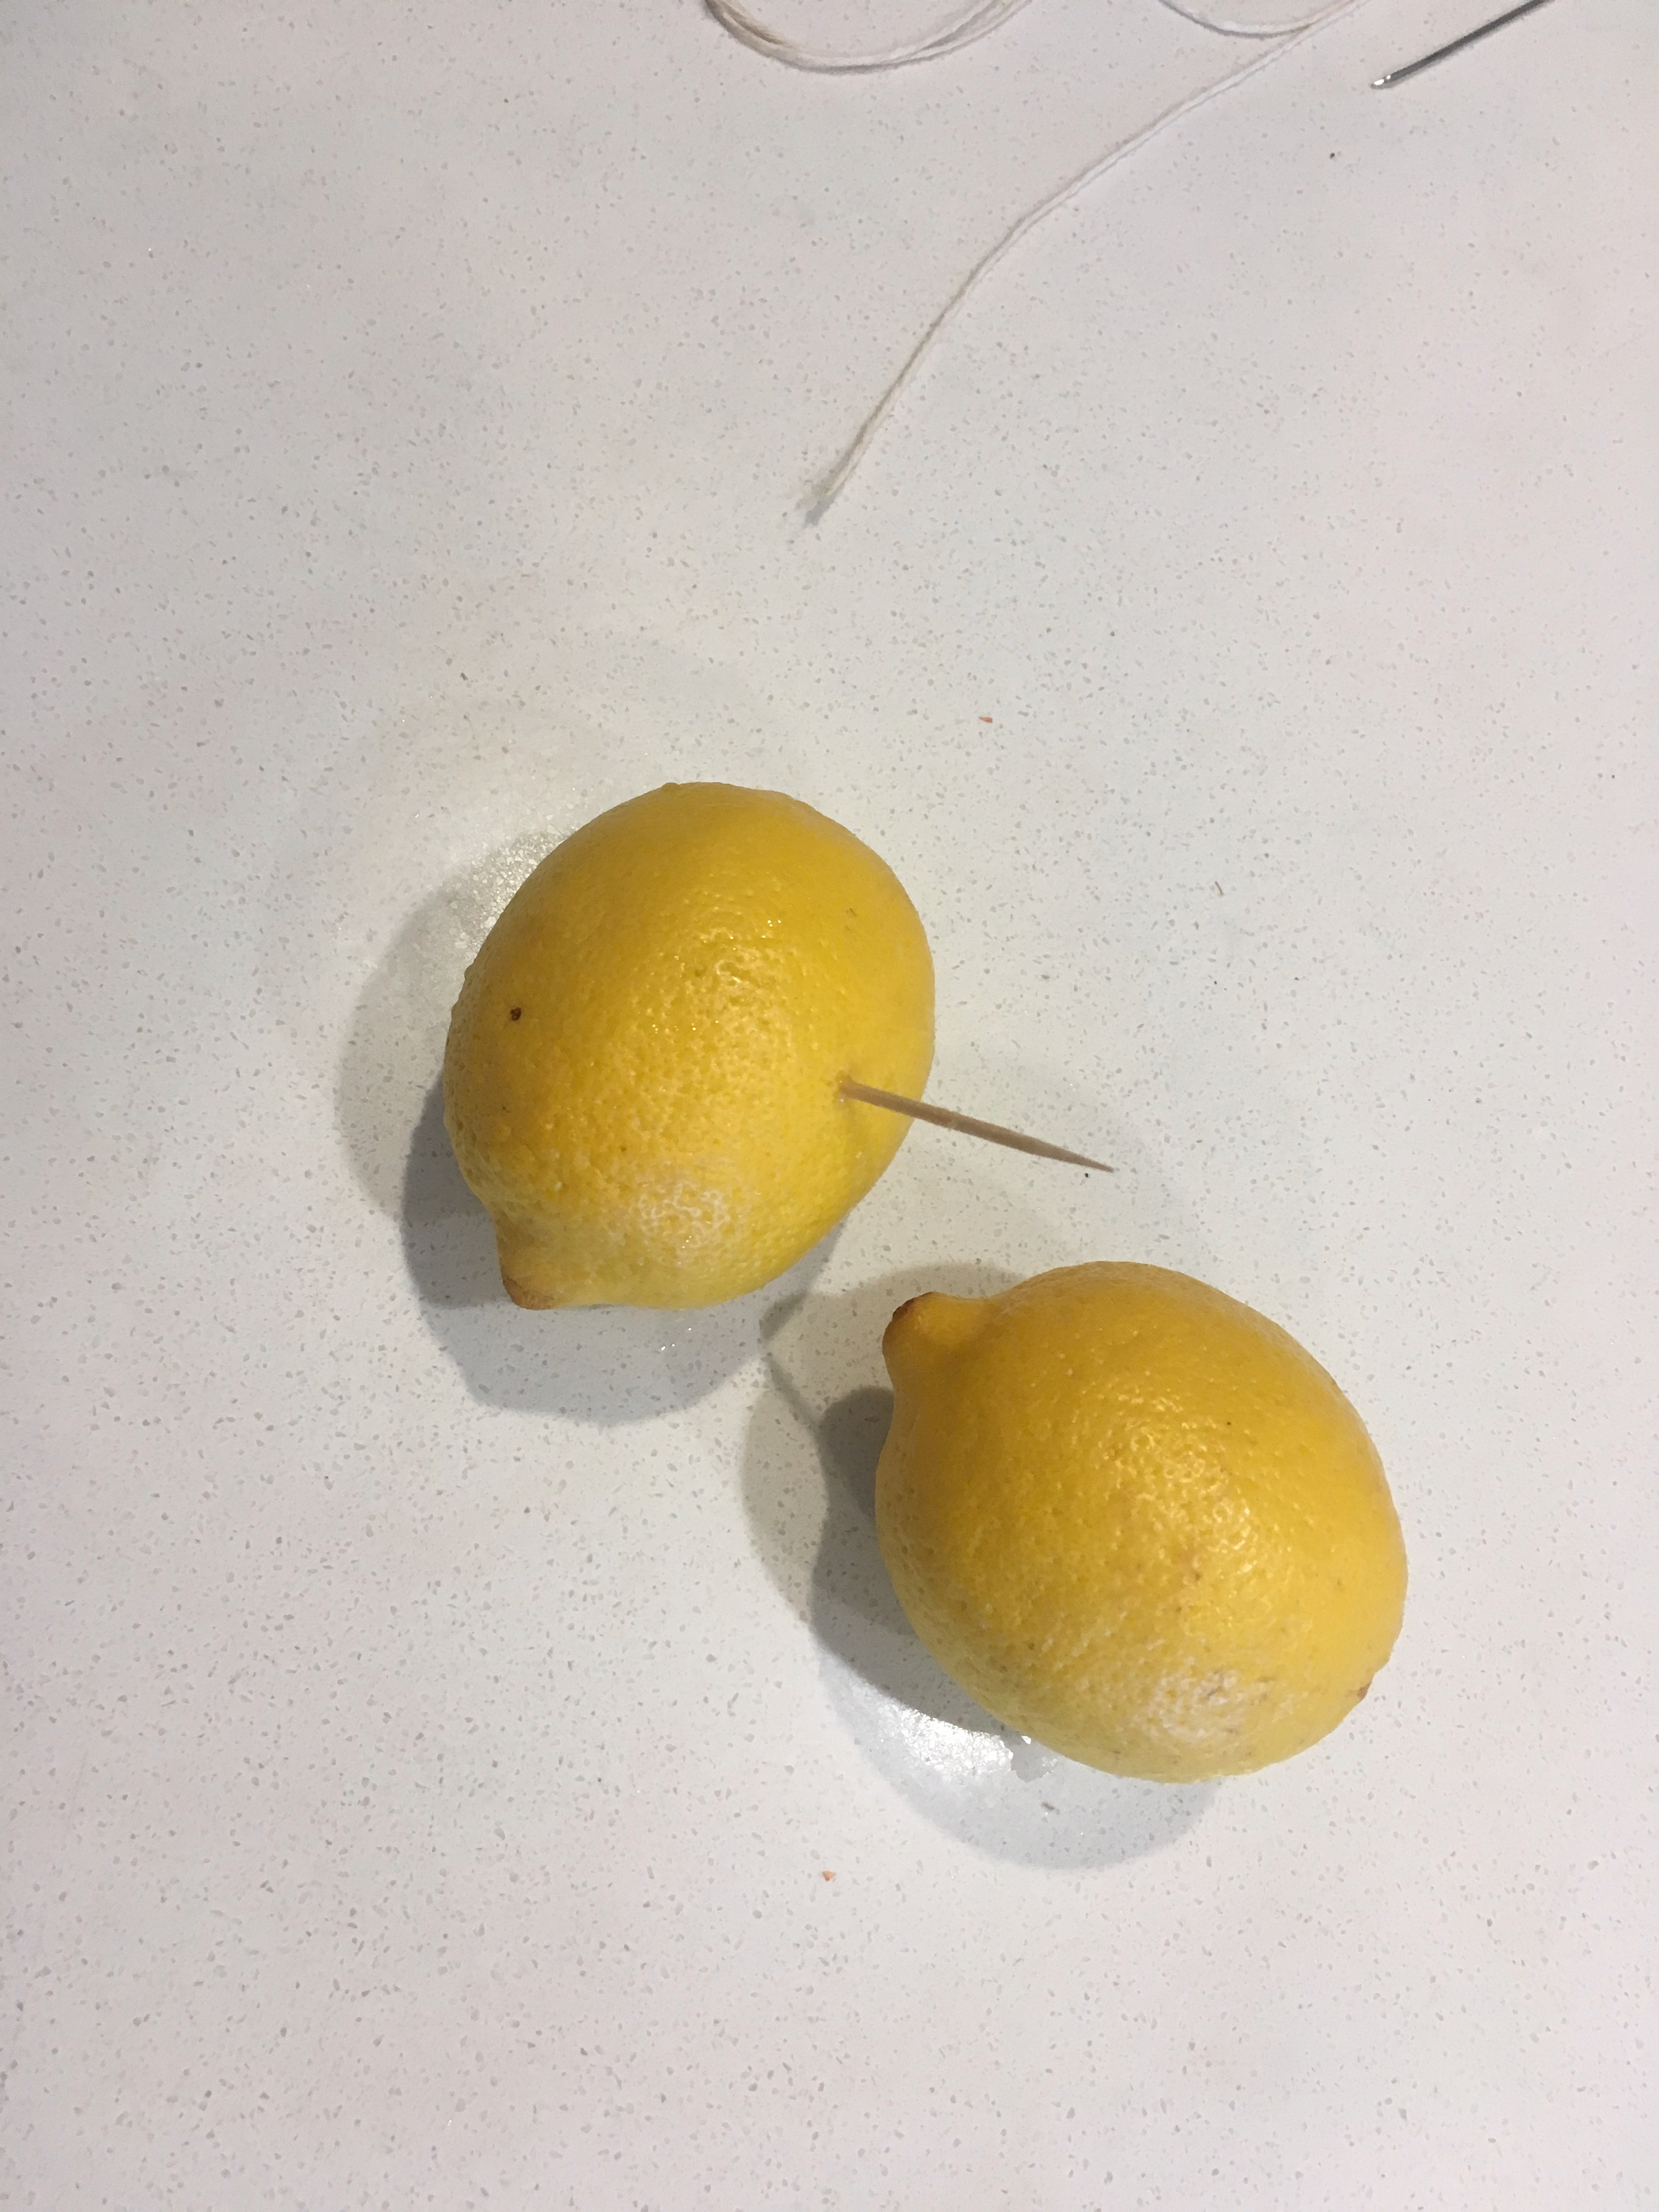
\includegraphics[width=0.25\textwidth]{\imageDir/\fileName/IMG_3212.jpg} &
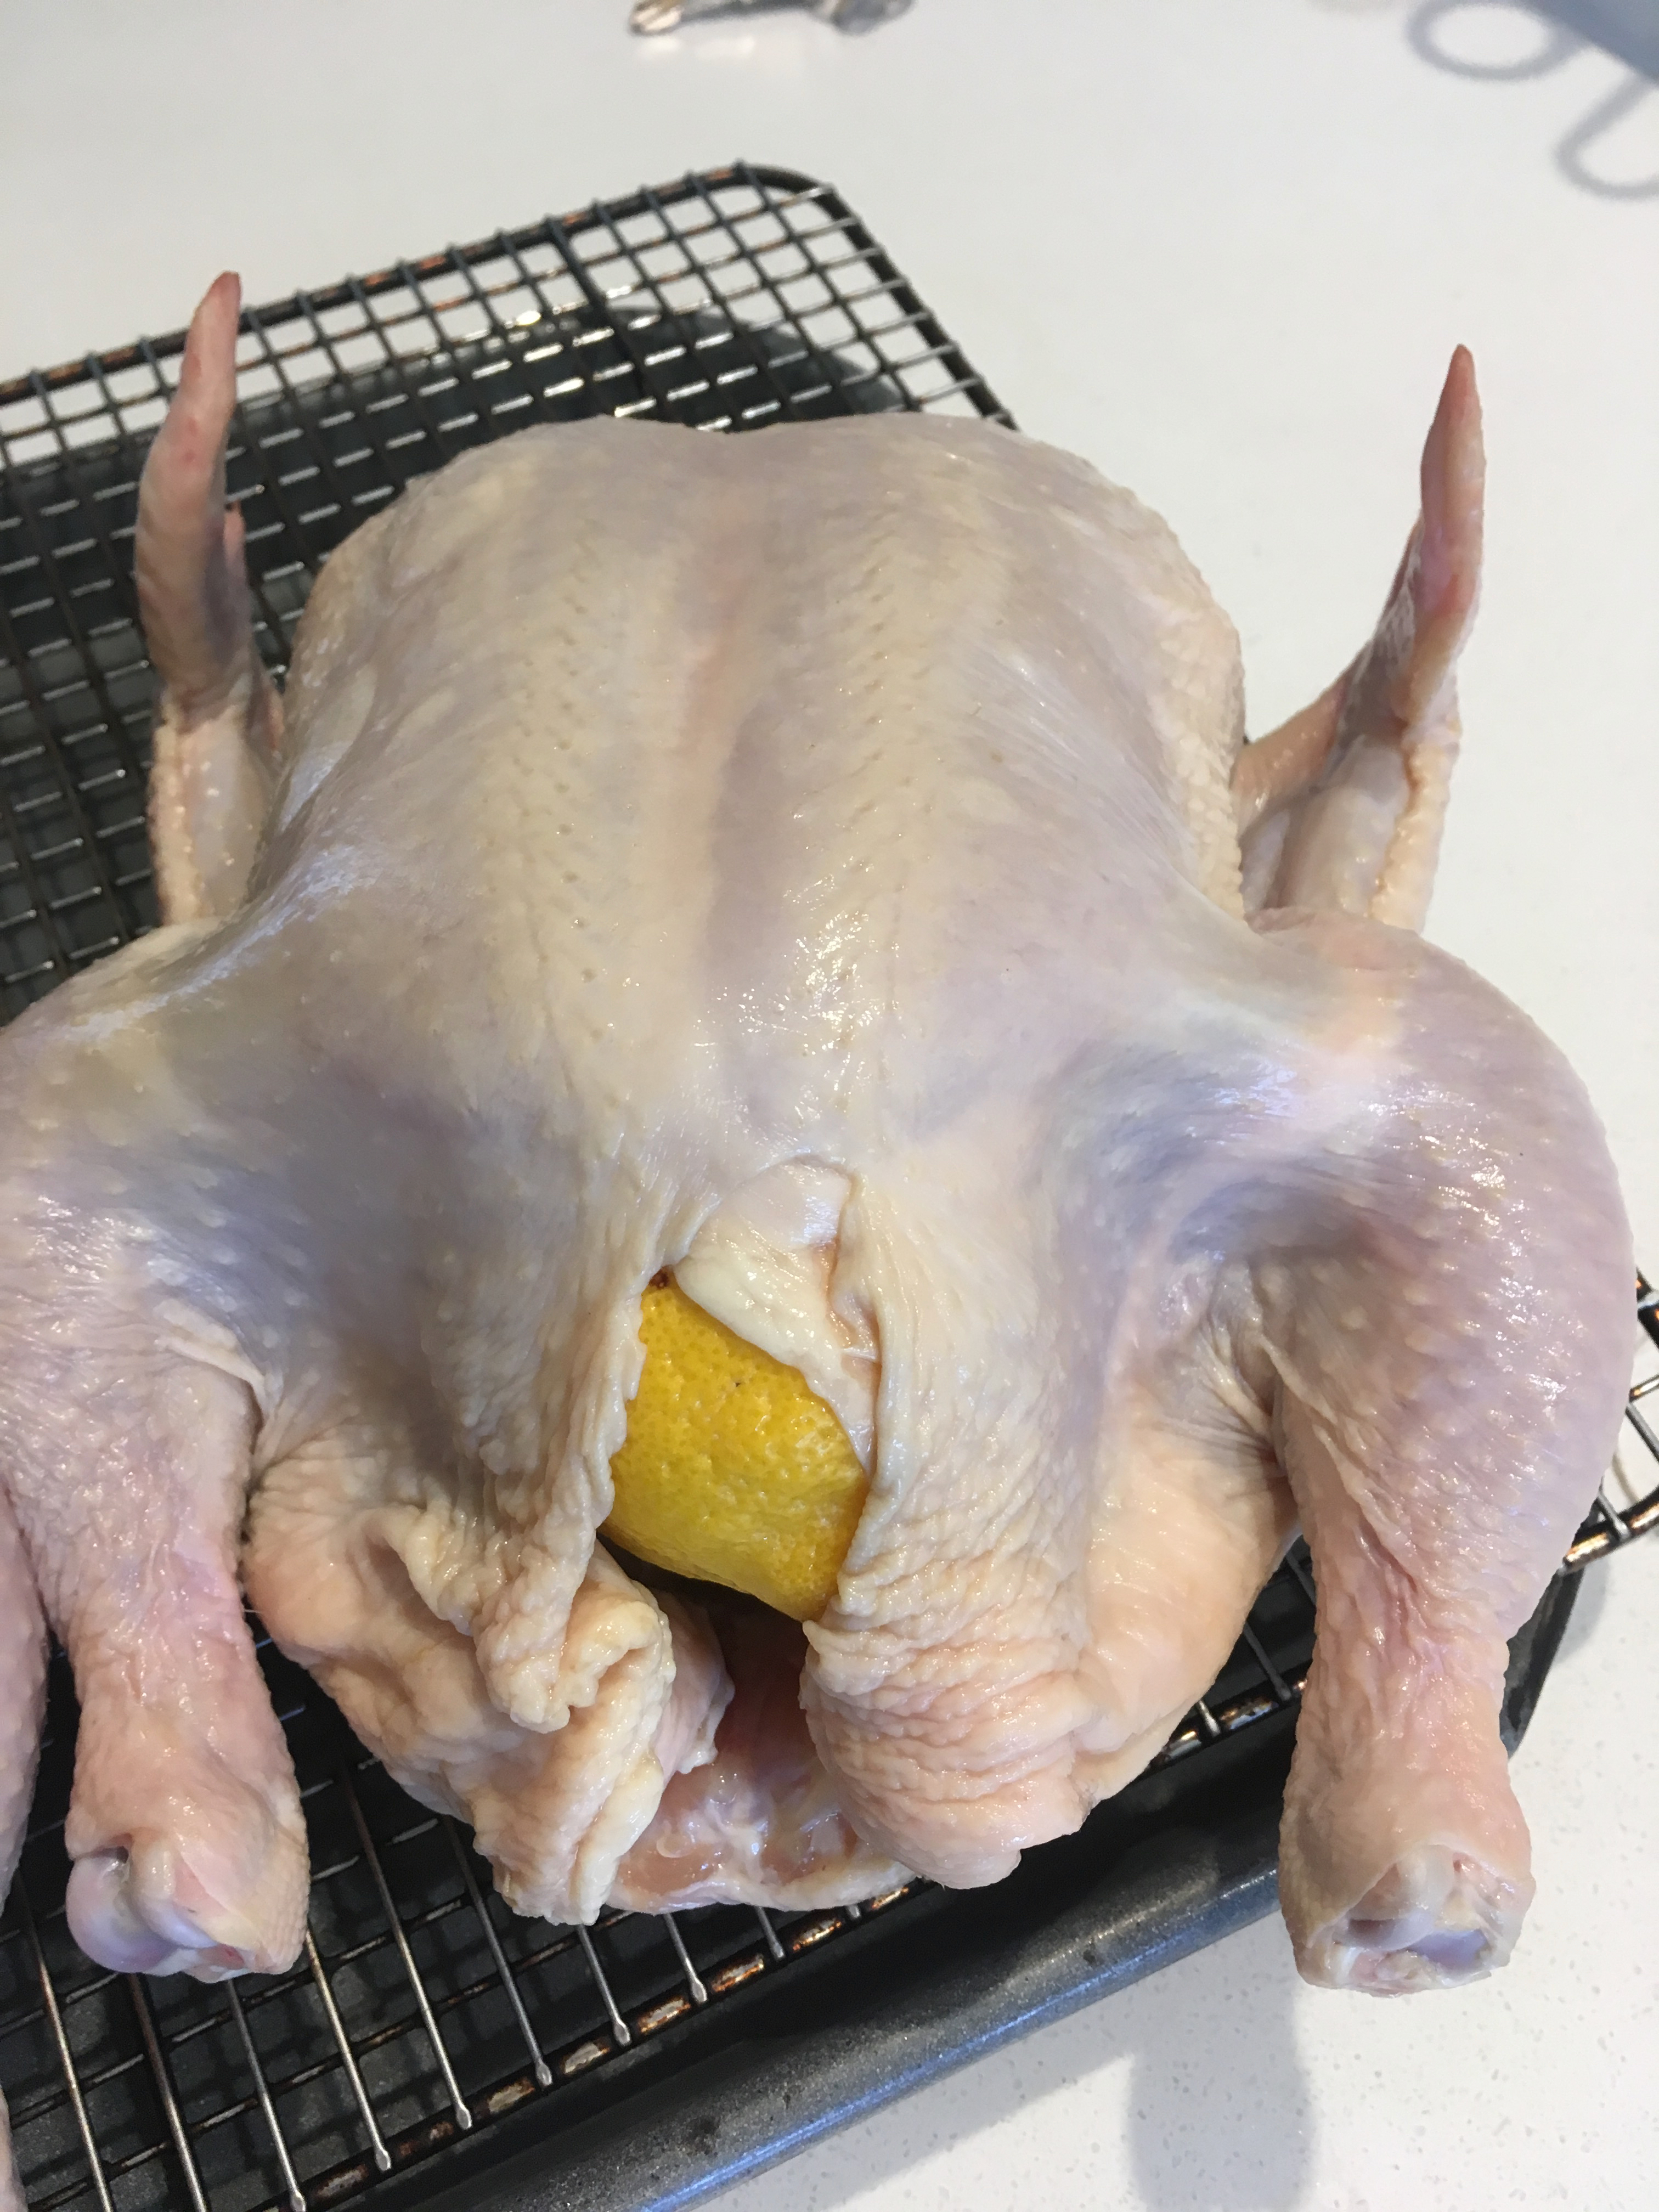
\includegraphics[width=0.25\textwidth]{\imageDir/\fileName/IMG_3213.jpg} \\
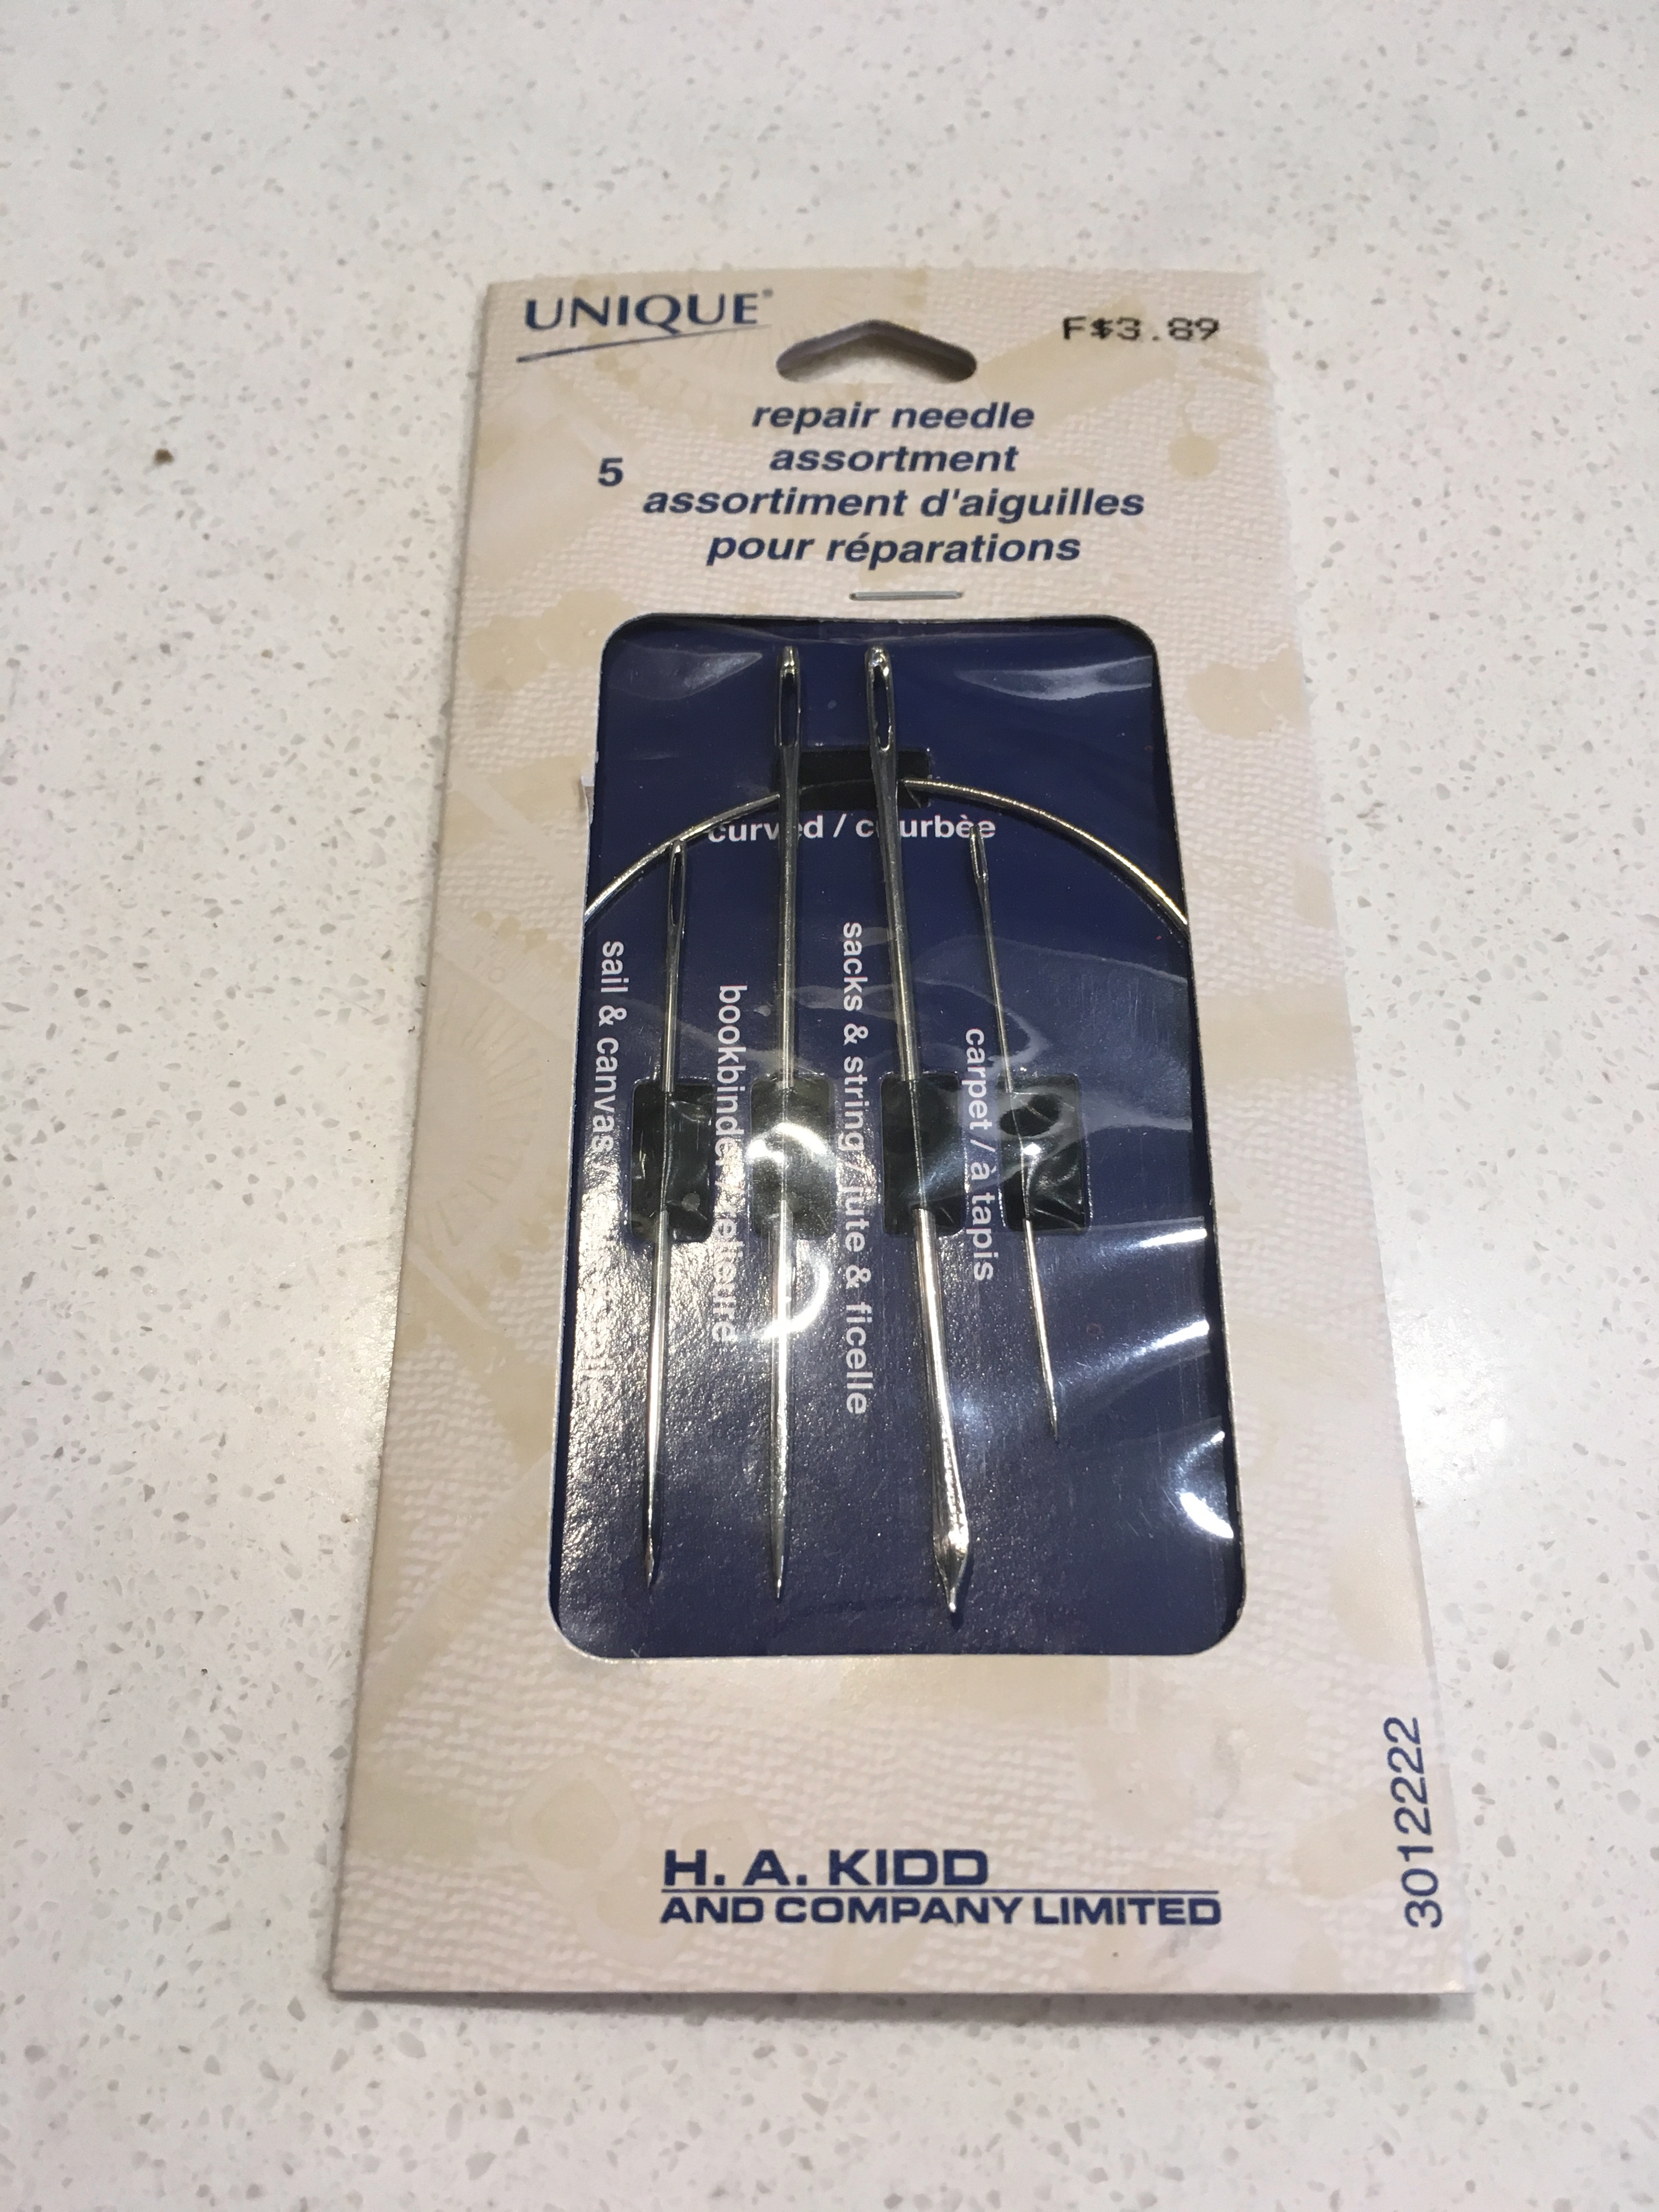
\includegraphics[width=0.25\textwidth]{\imageDir/\fileName/IMG_3206.jpg} &
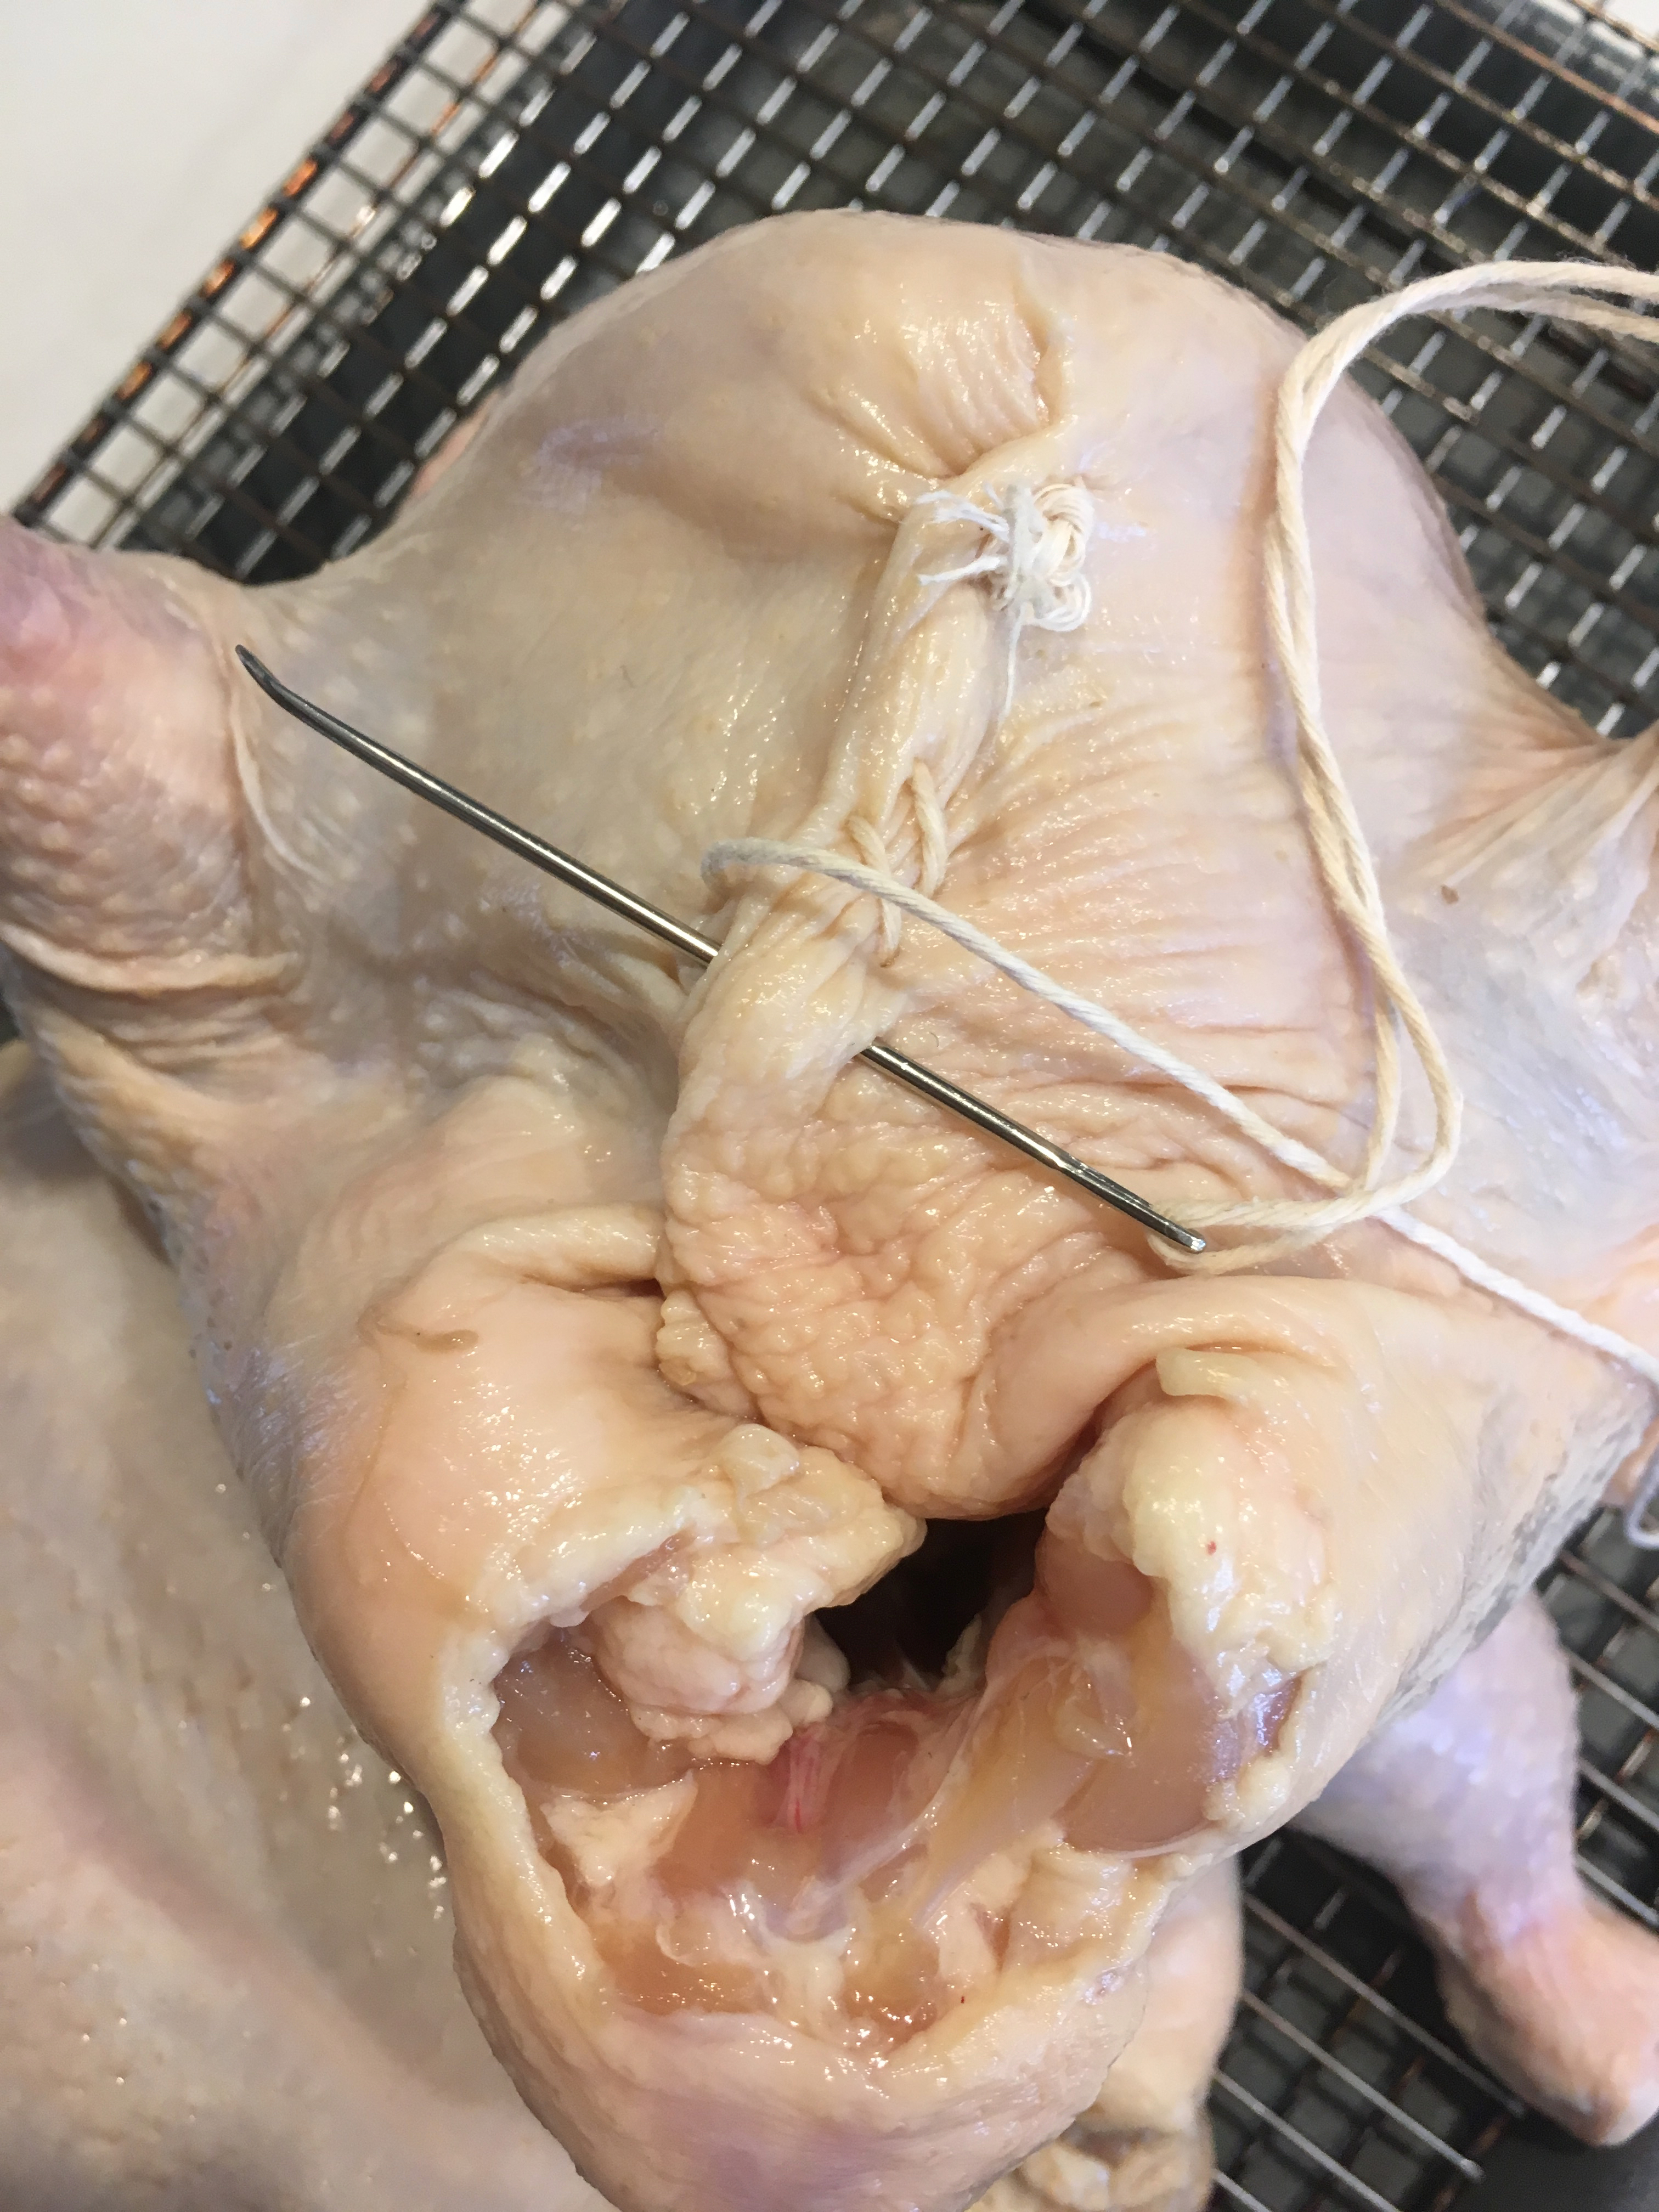
\includegraphics[width=0.25\textwidth]{\imageDir/\fileName/IMG_3214.jpg} &
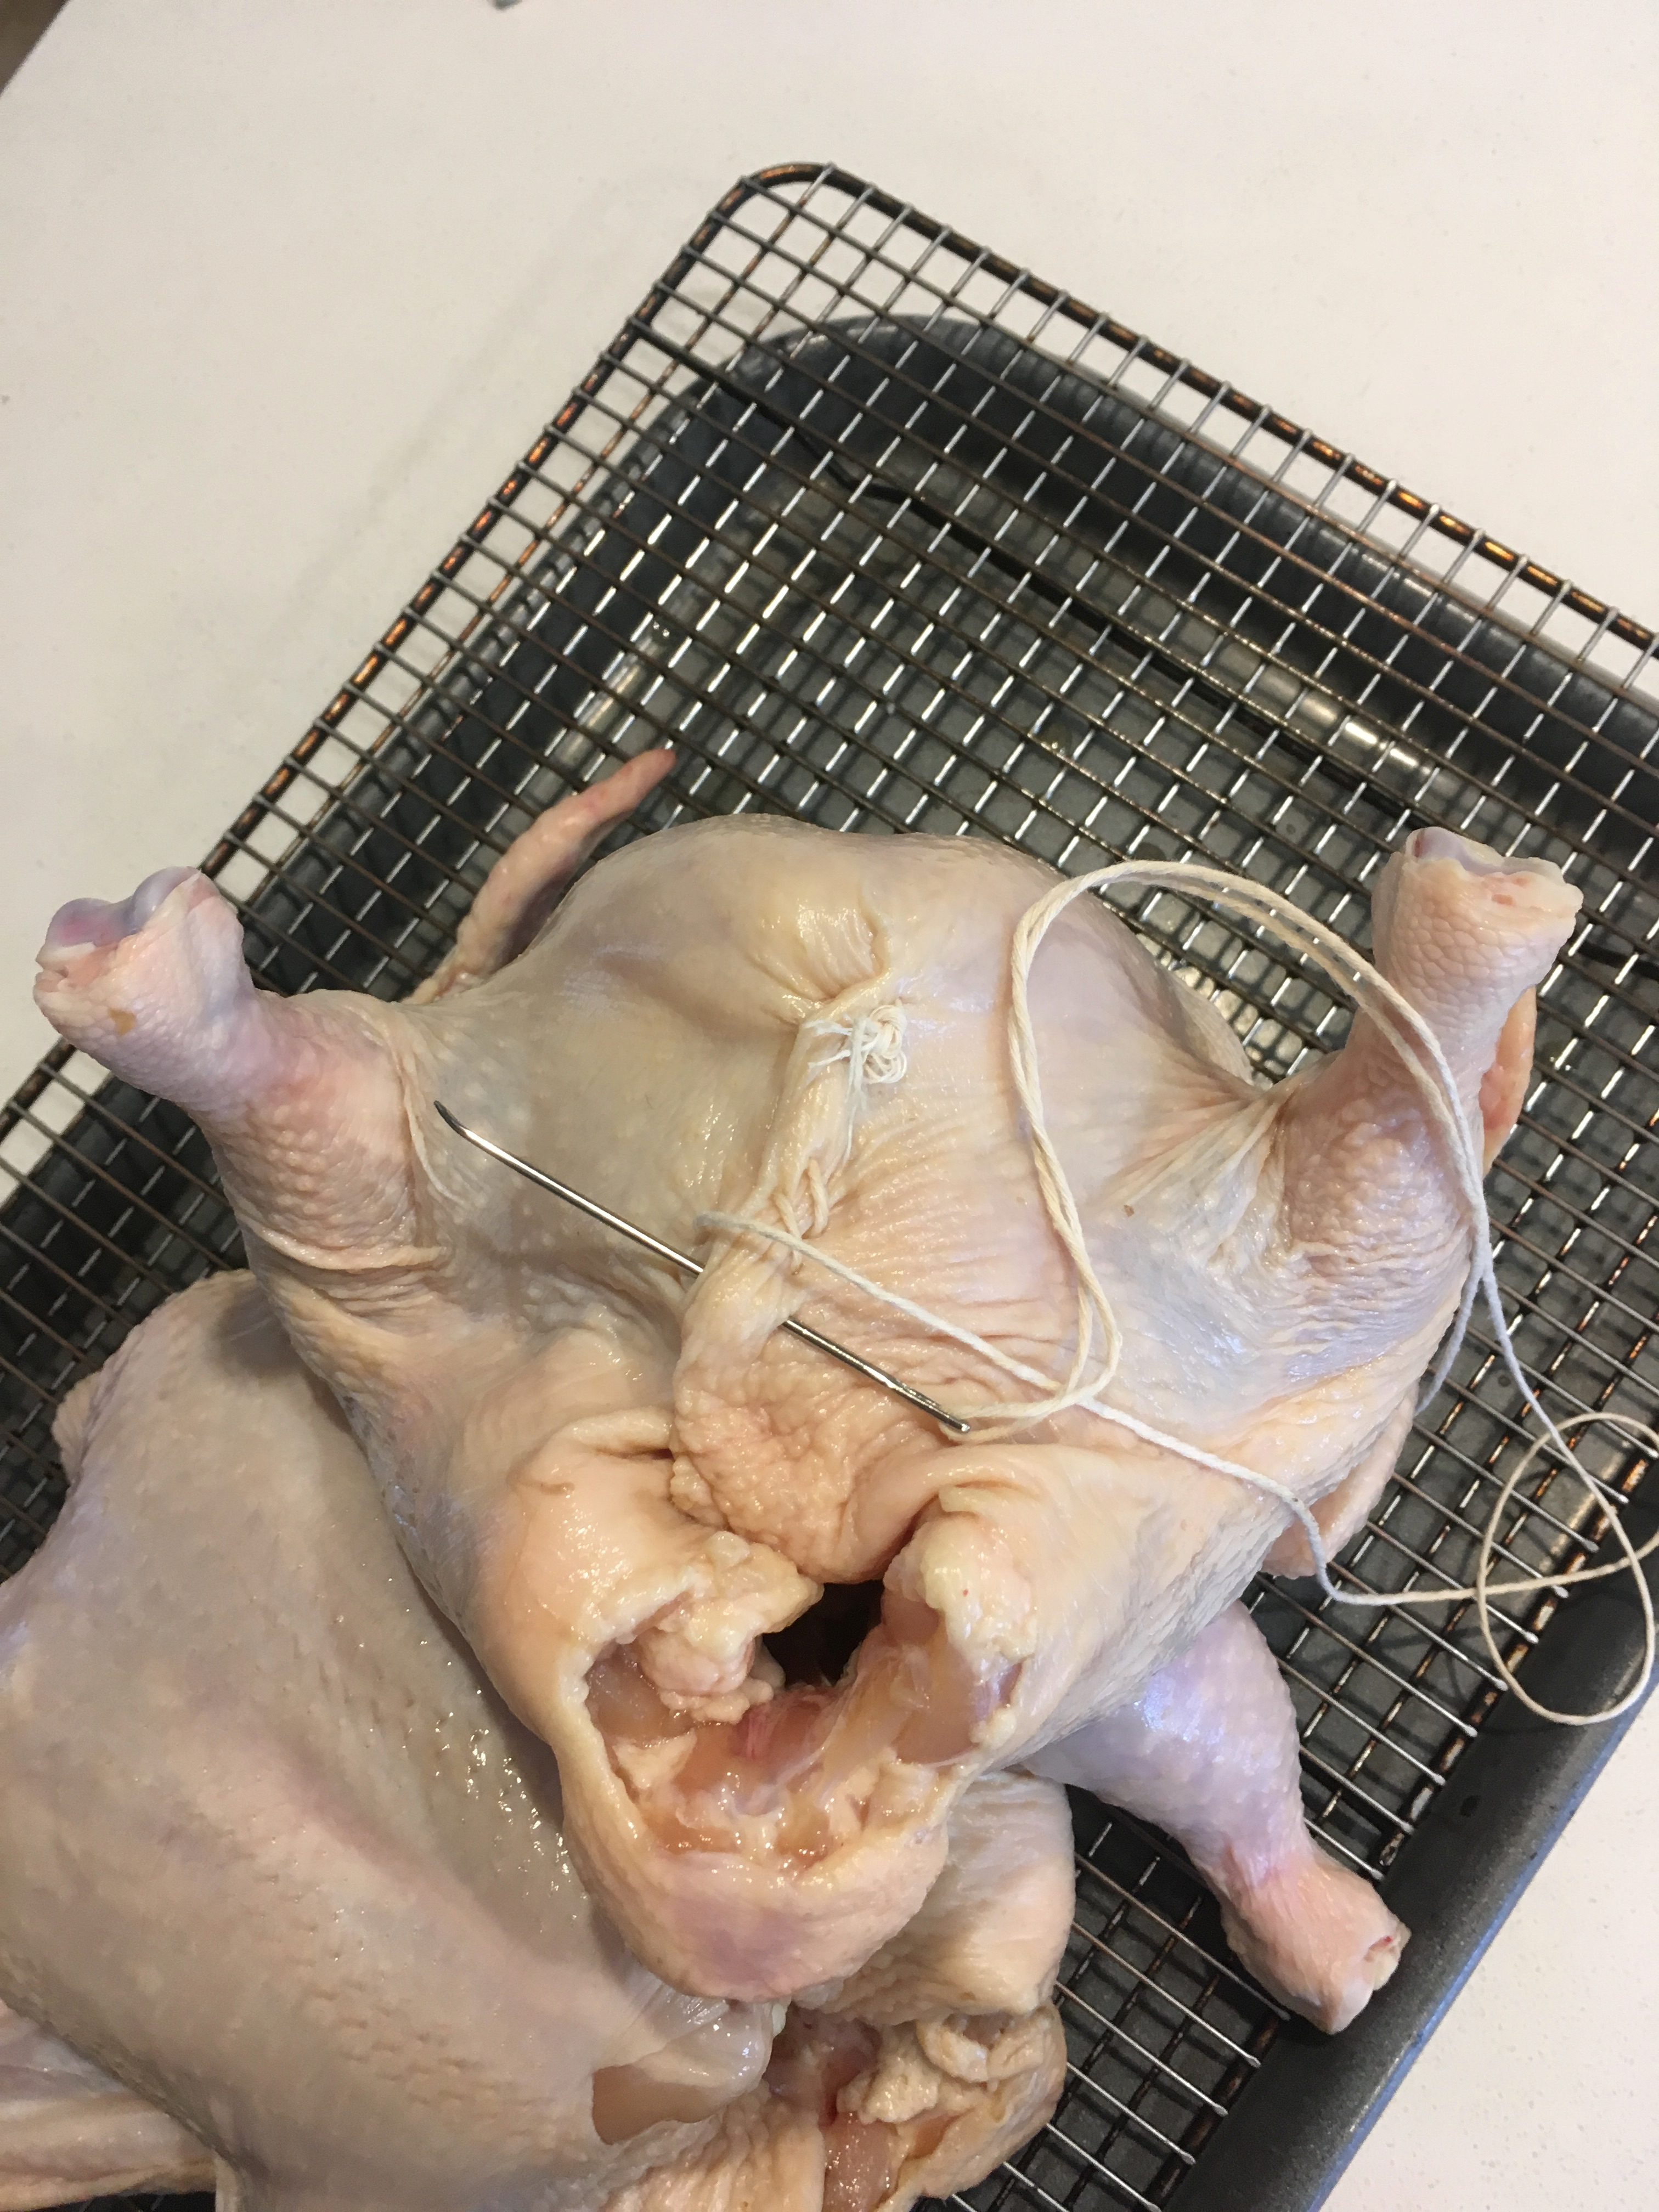
\includegraphics[width=0.25\textwidth]{\imageDir/\fileName/IMG_3216.jpg} \\
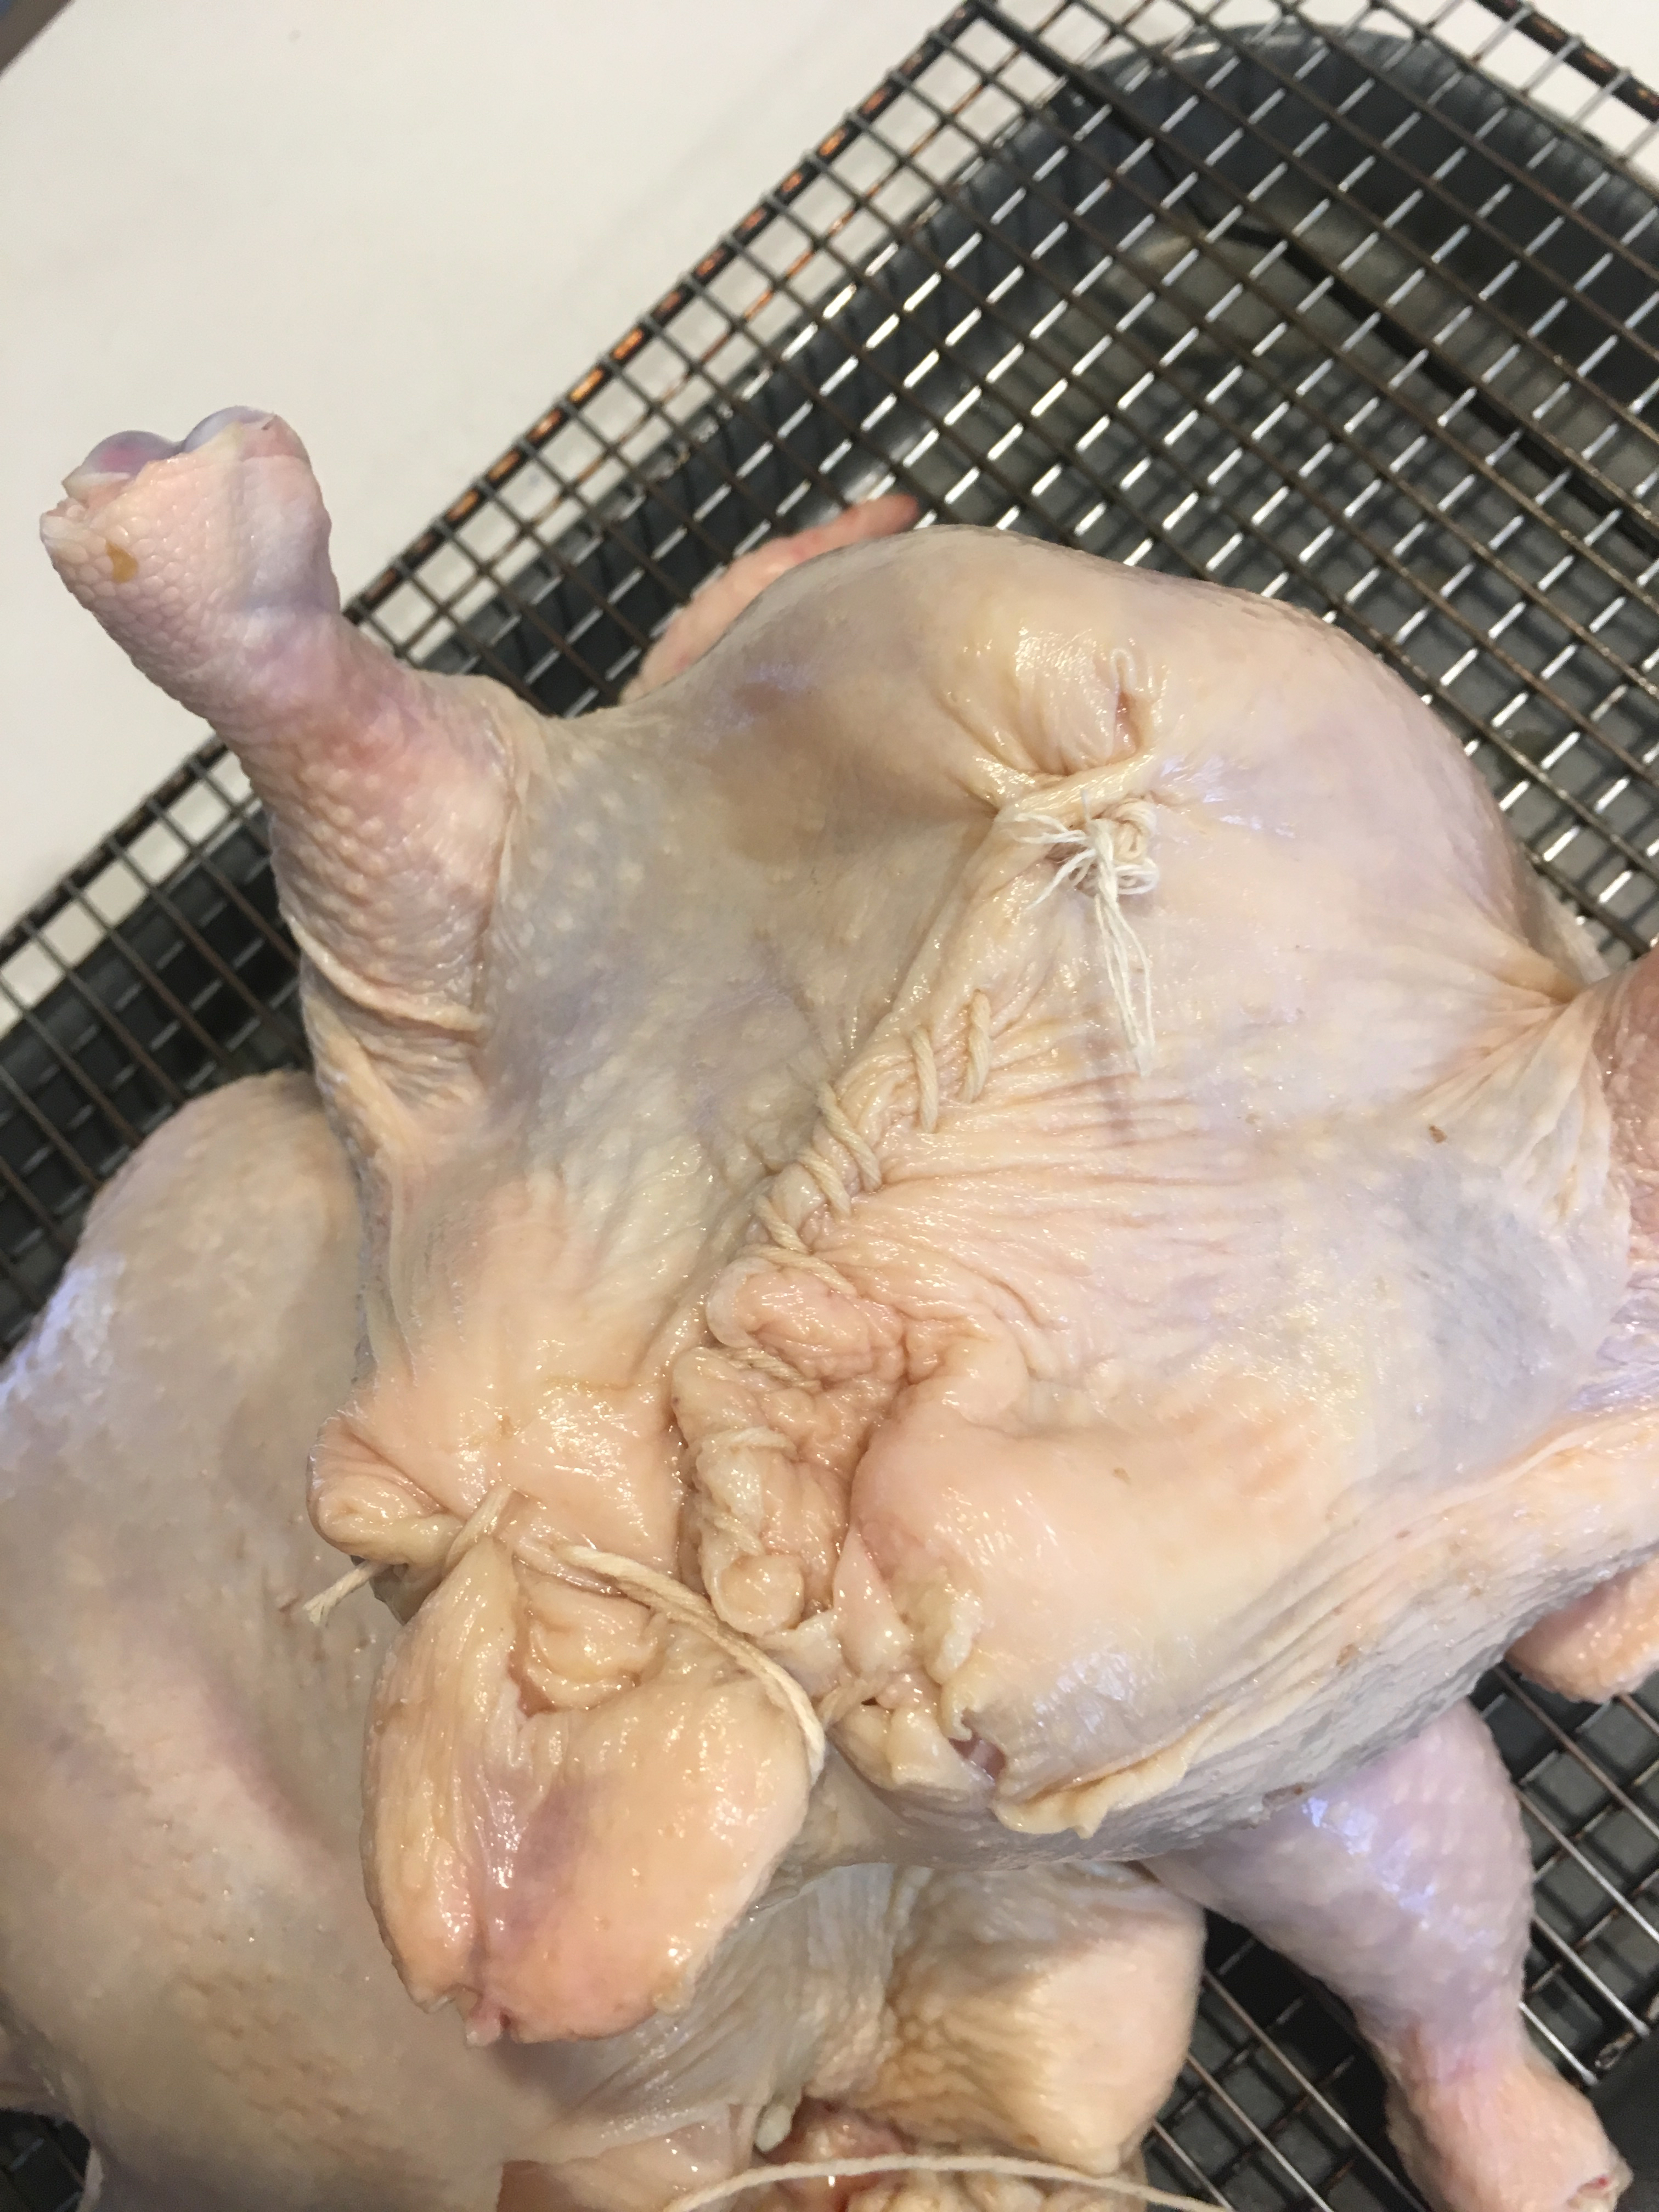
\includegraphics[width=0.25\textwidth]{\imageDir/\fileName/IMG_3217.jpg} &
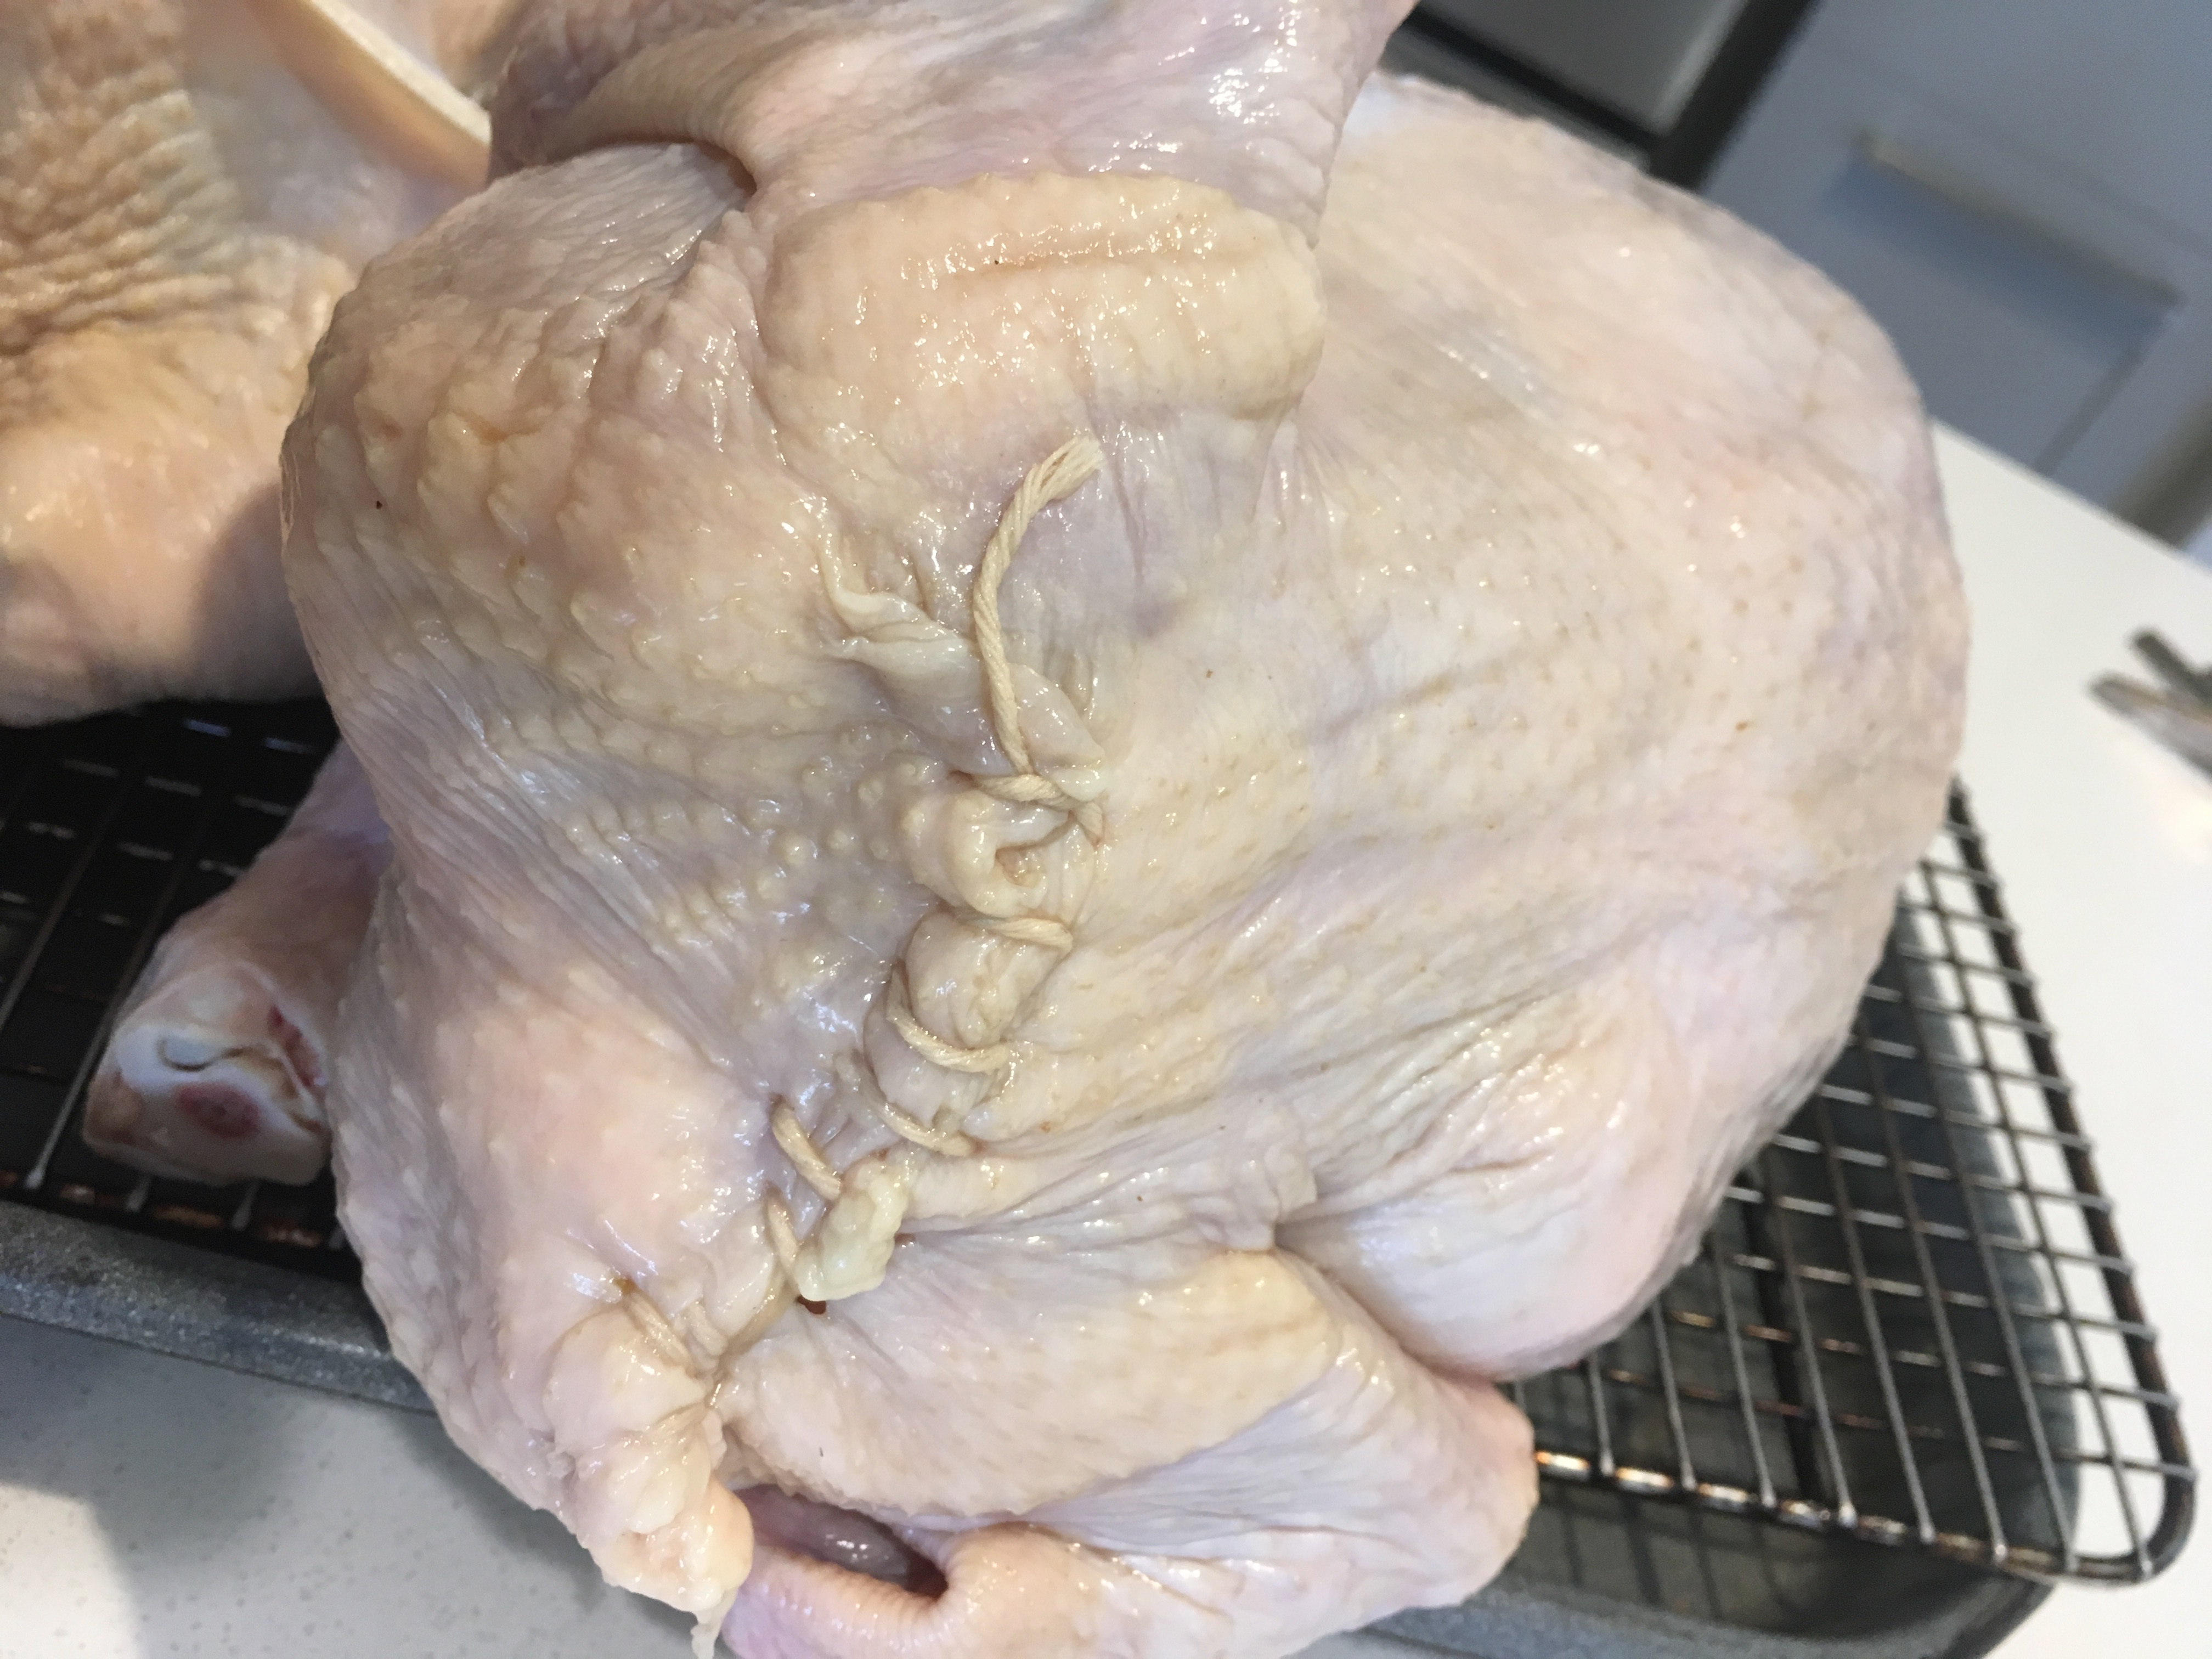
\includegraphics[width=0.25\textwidth]{\imageDir/\fileName/IMG_3218.jpg} &
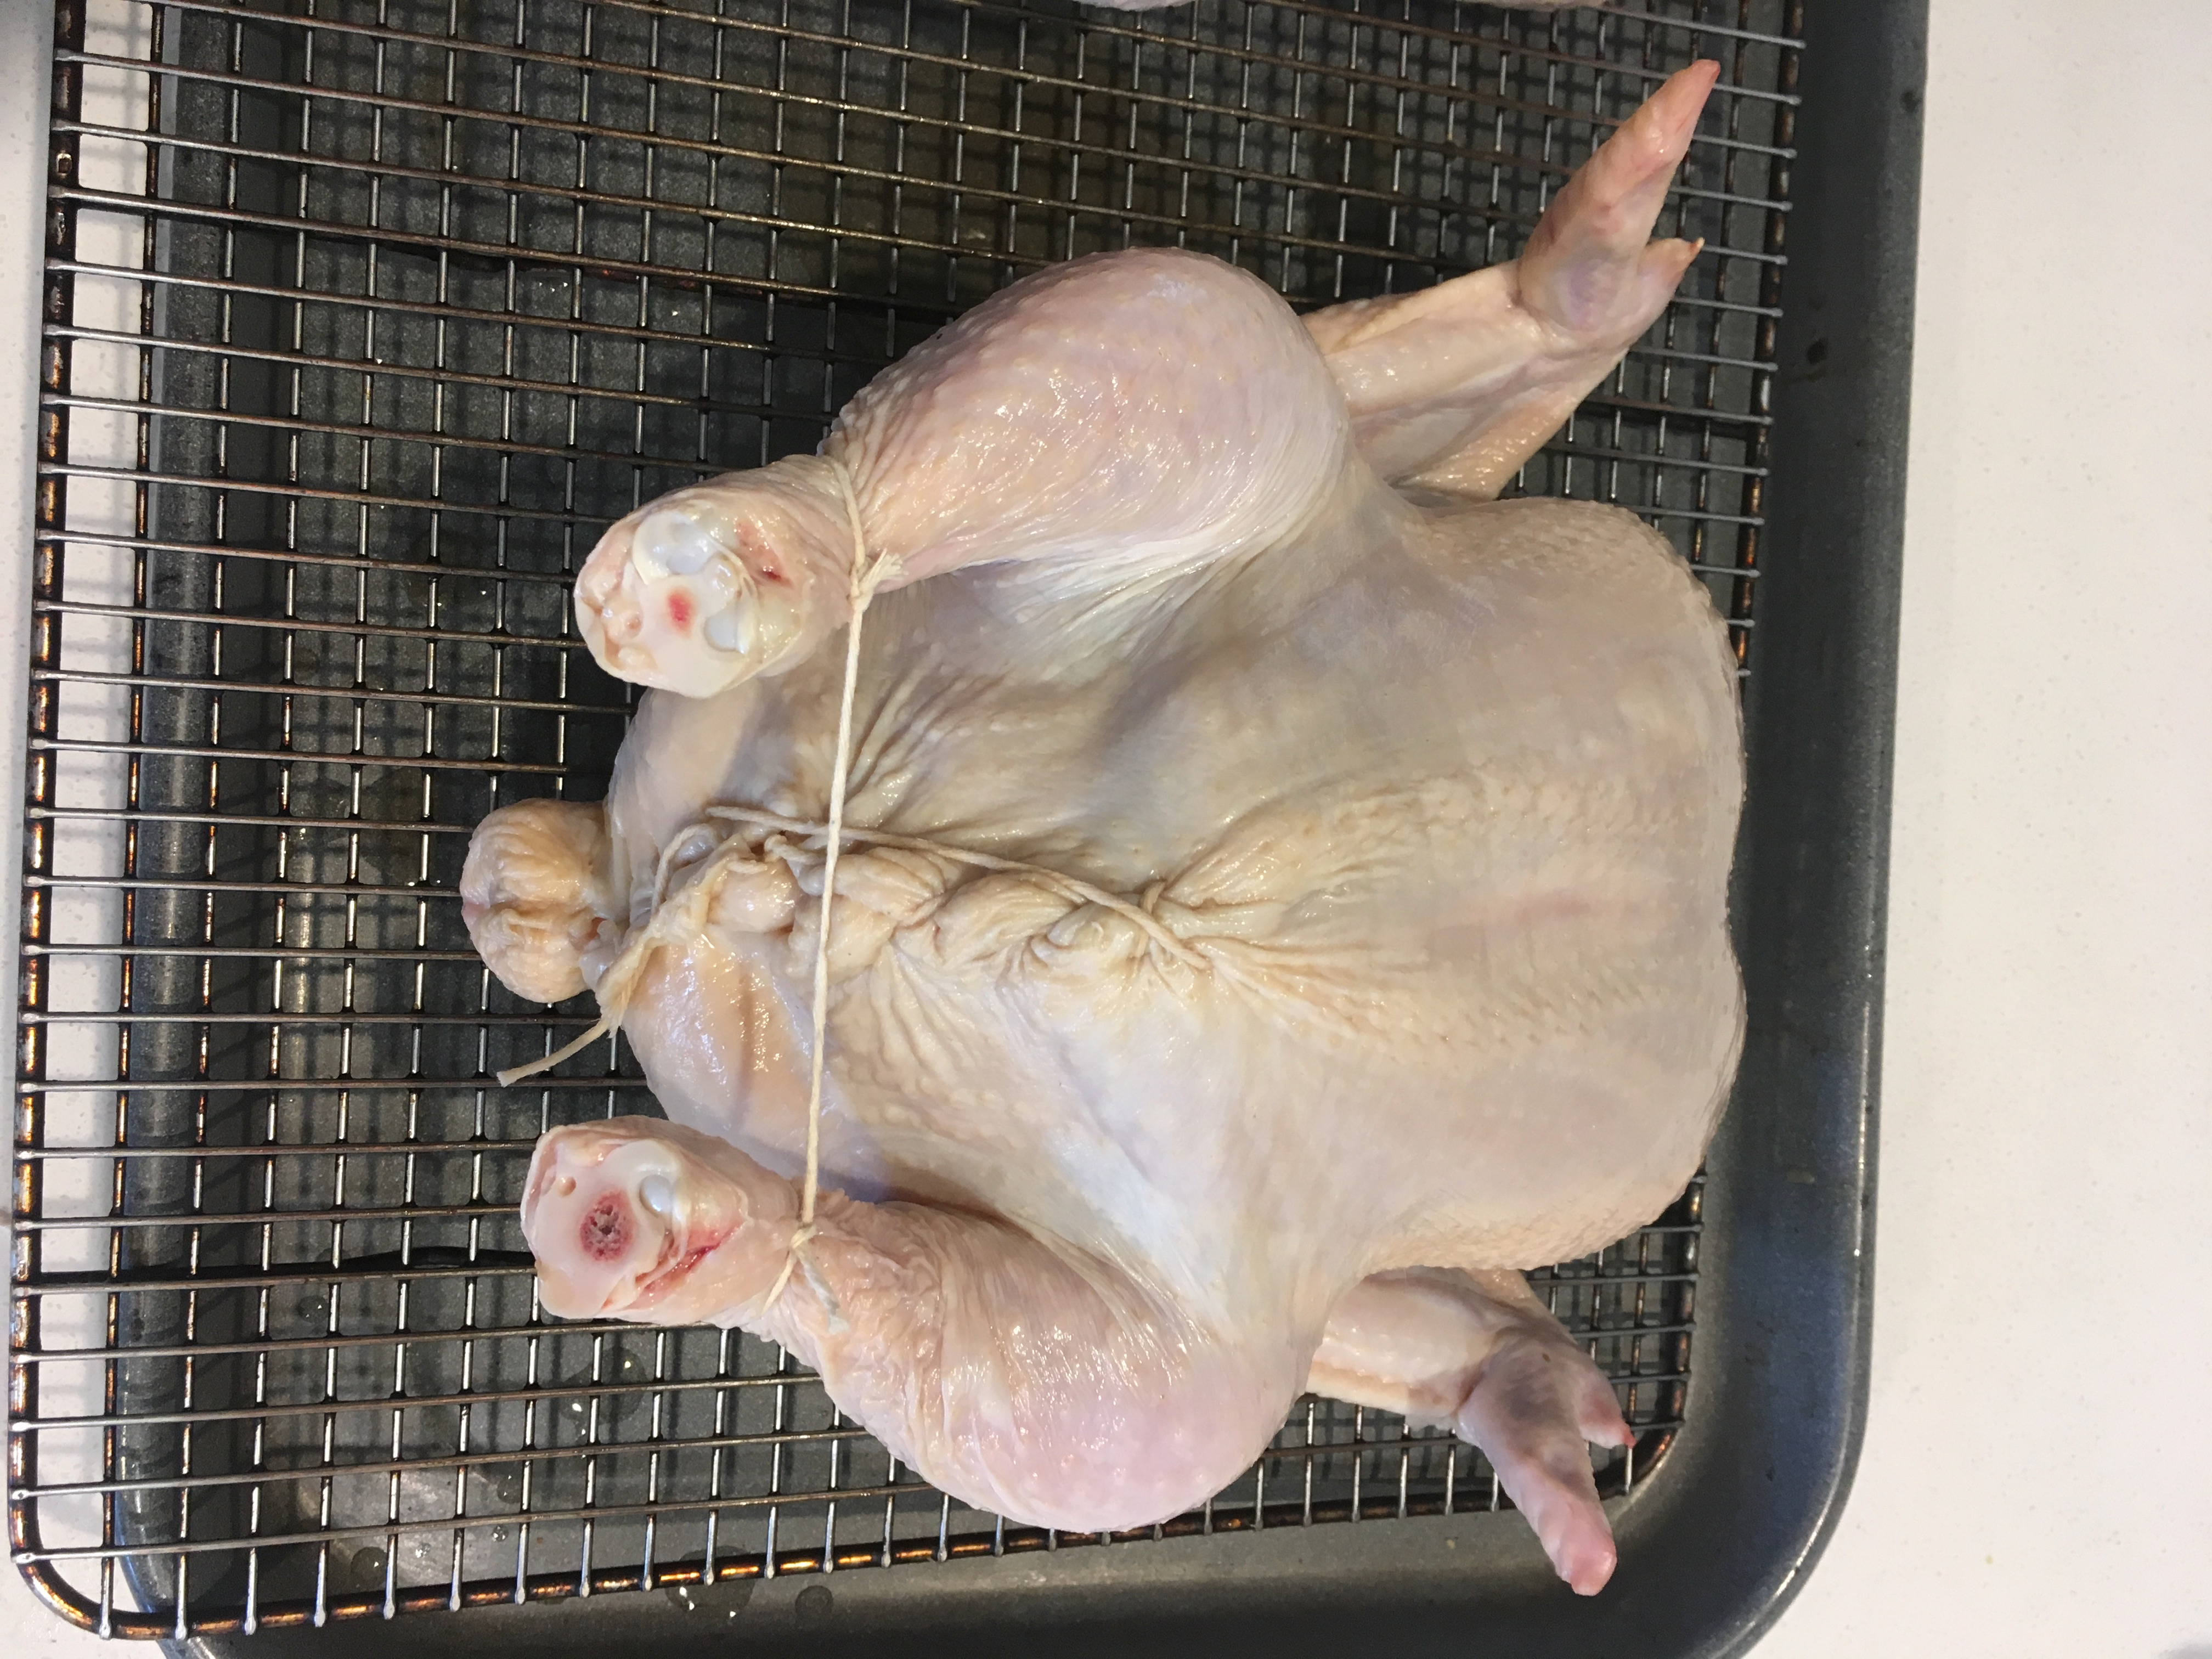
\includegraphics[width=0.25\textwidth]{\imageDir/\fileName/IMG_3219.jpg} \\
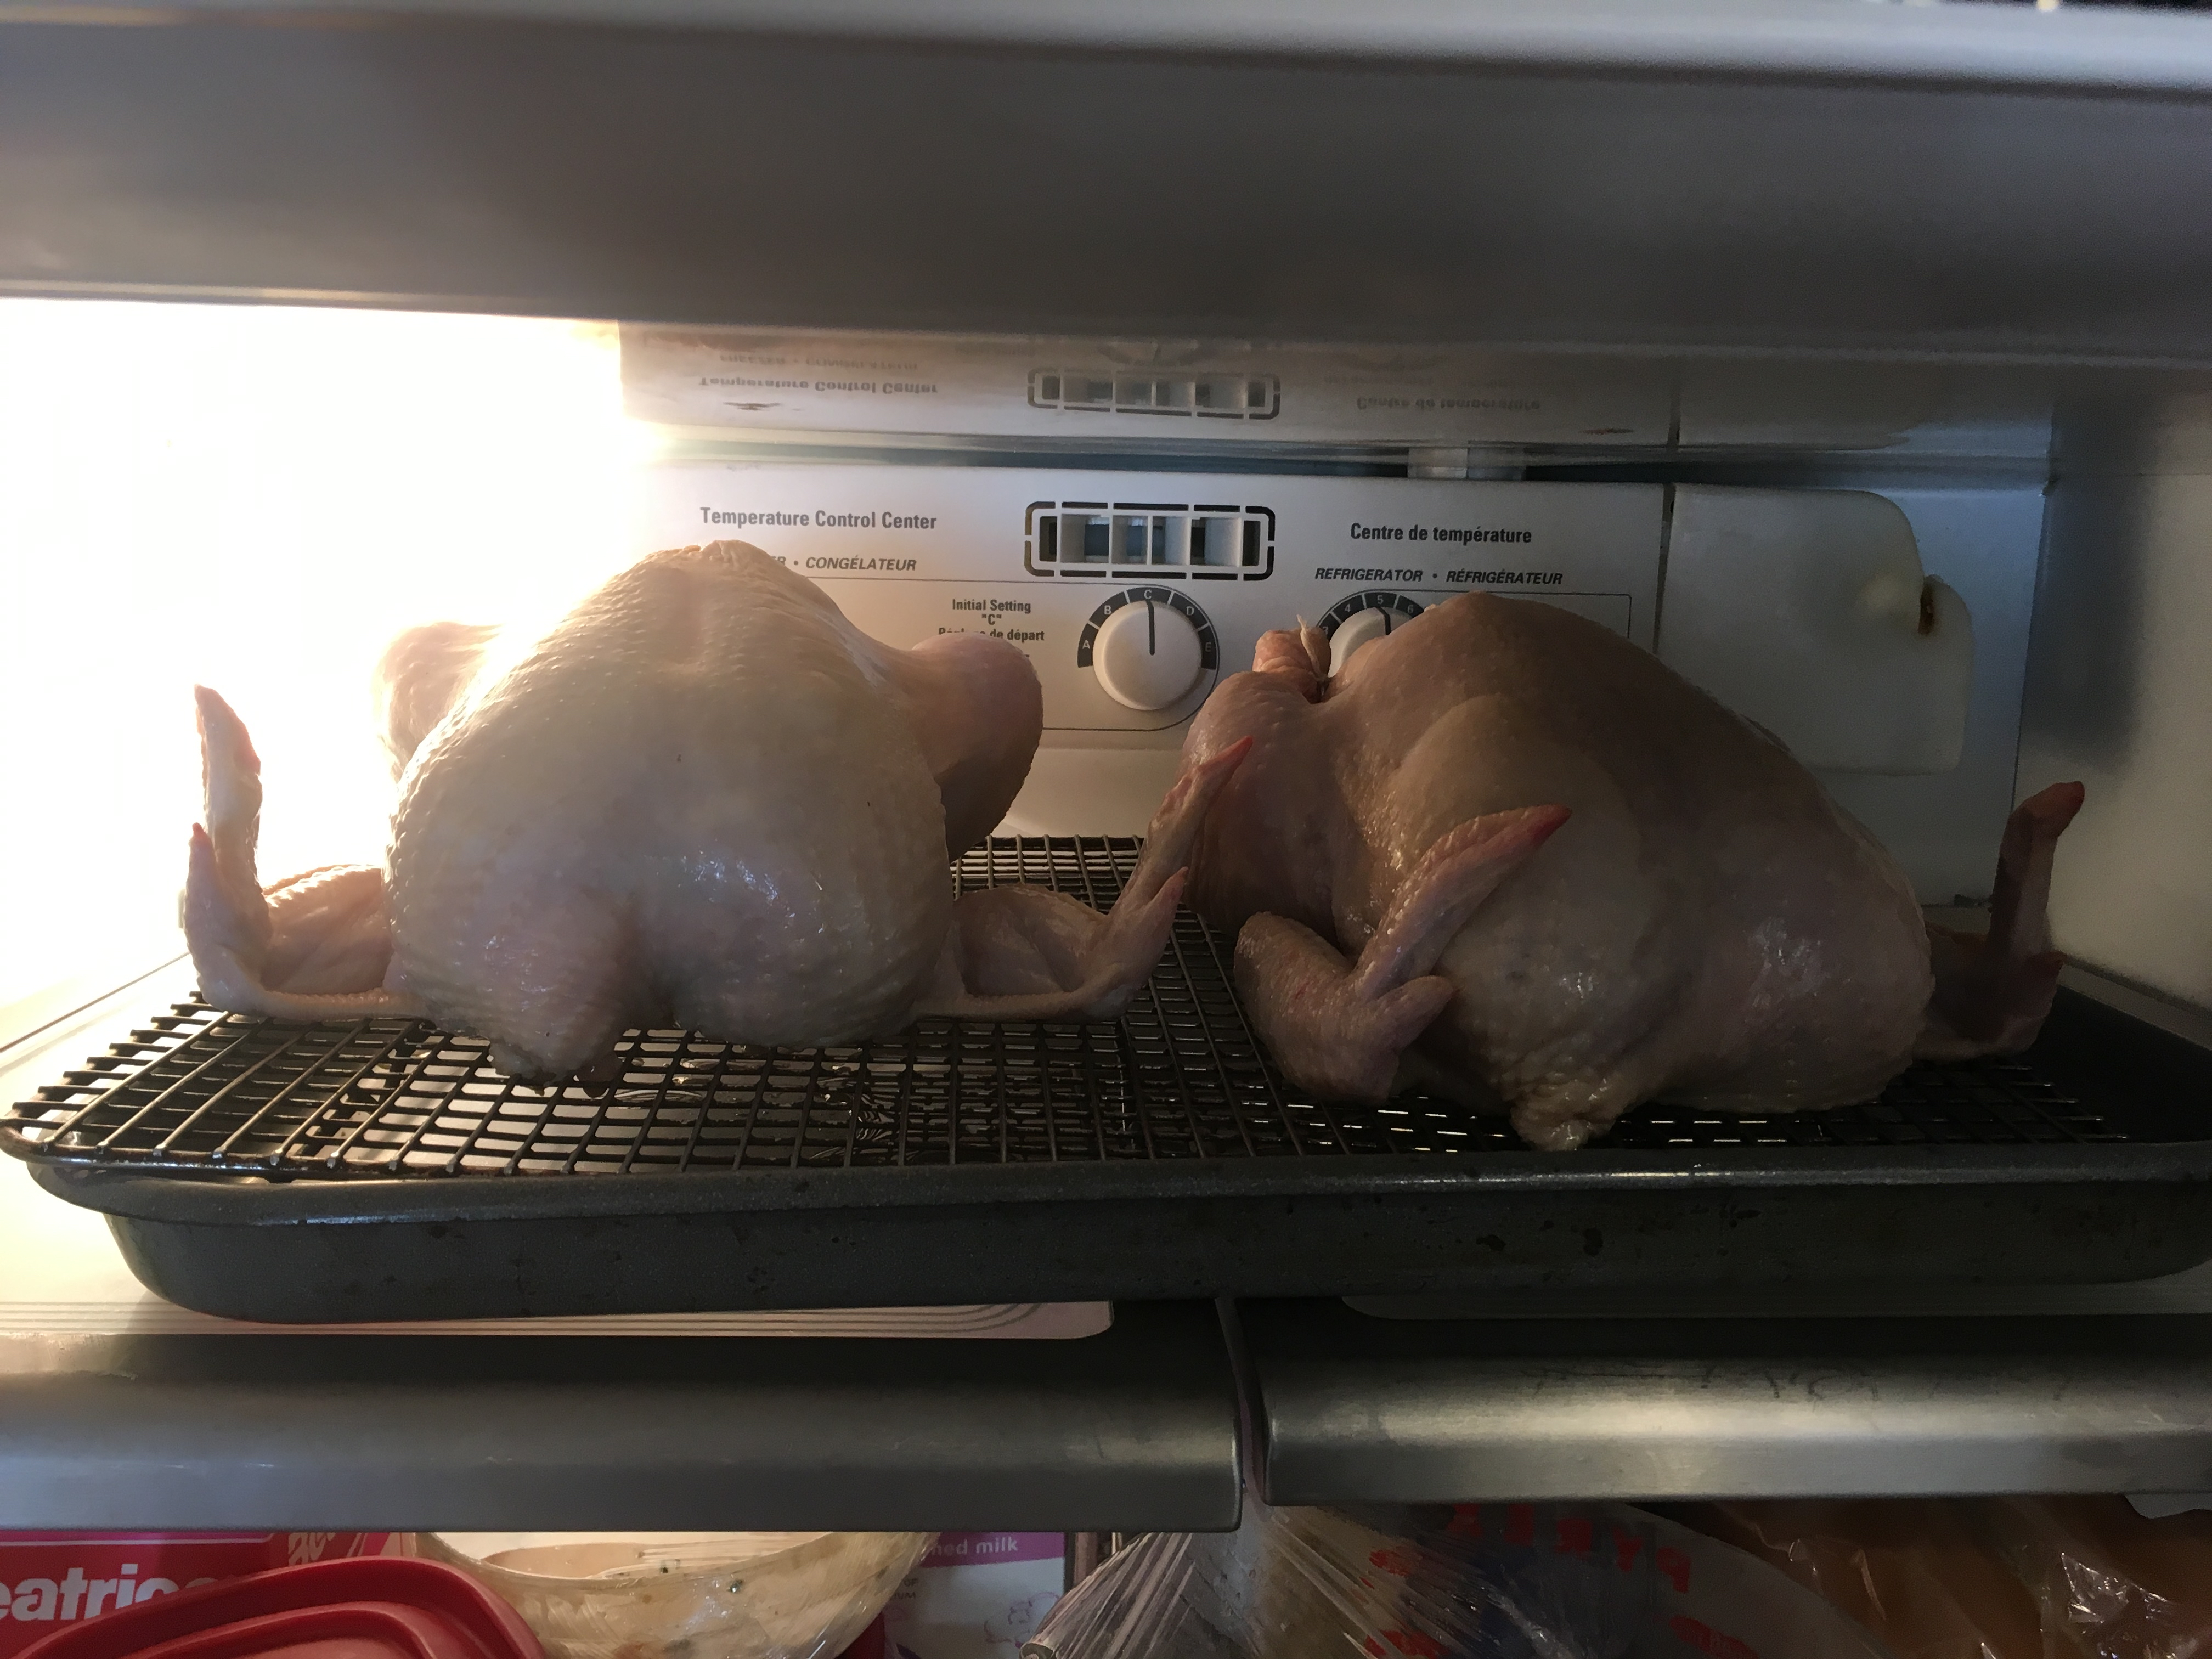
\includegraphics[width=0.25\textwidth]{\imageDir/\fileName/IMG_3220.jpg} &
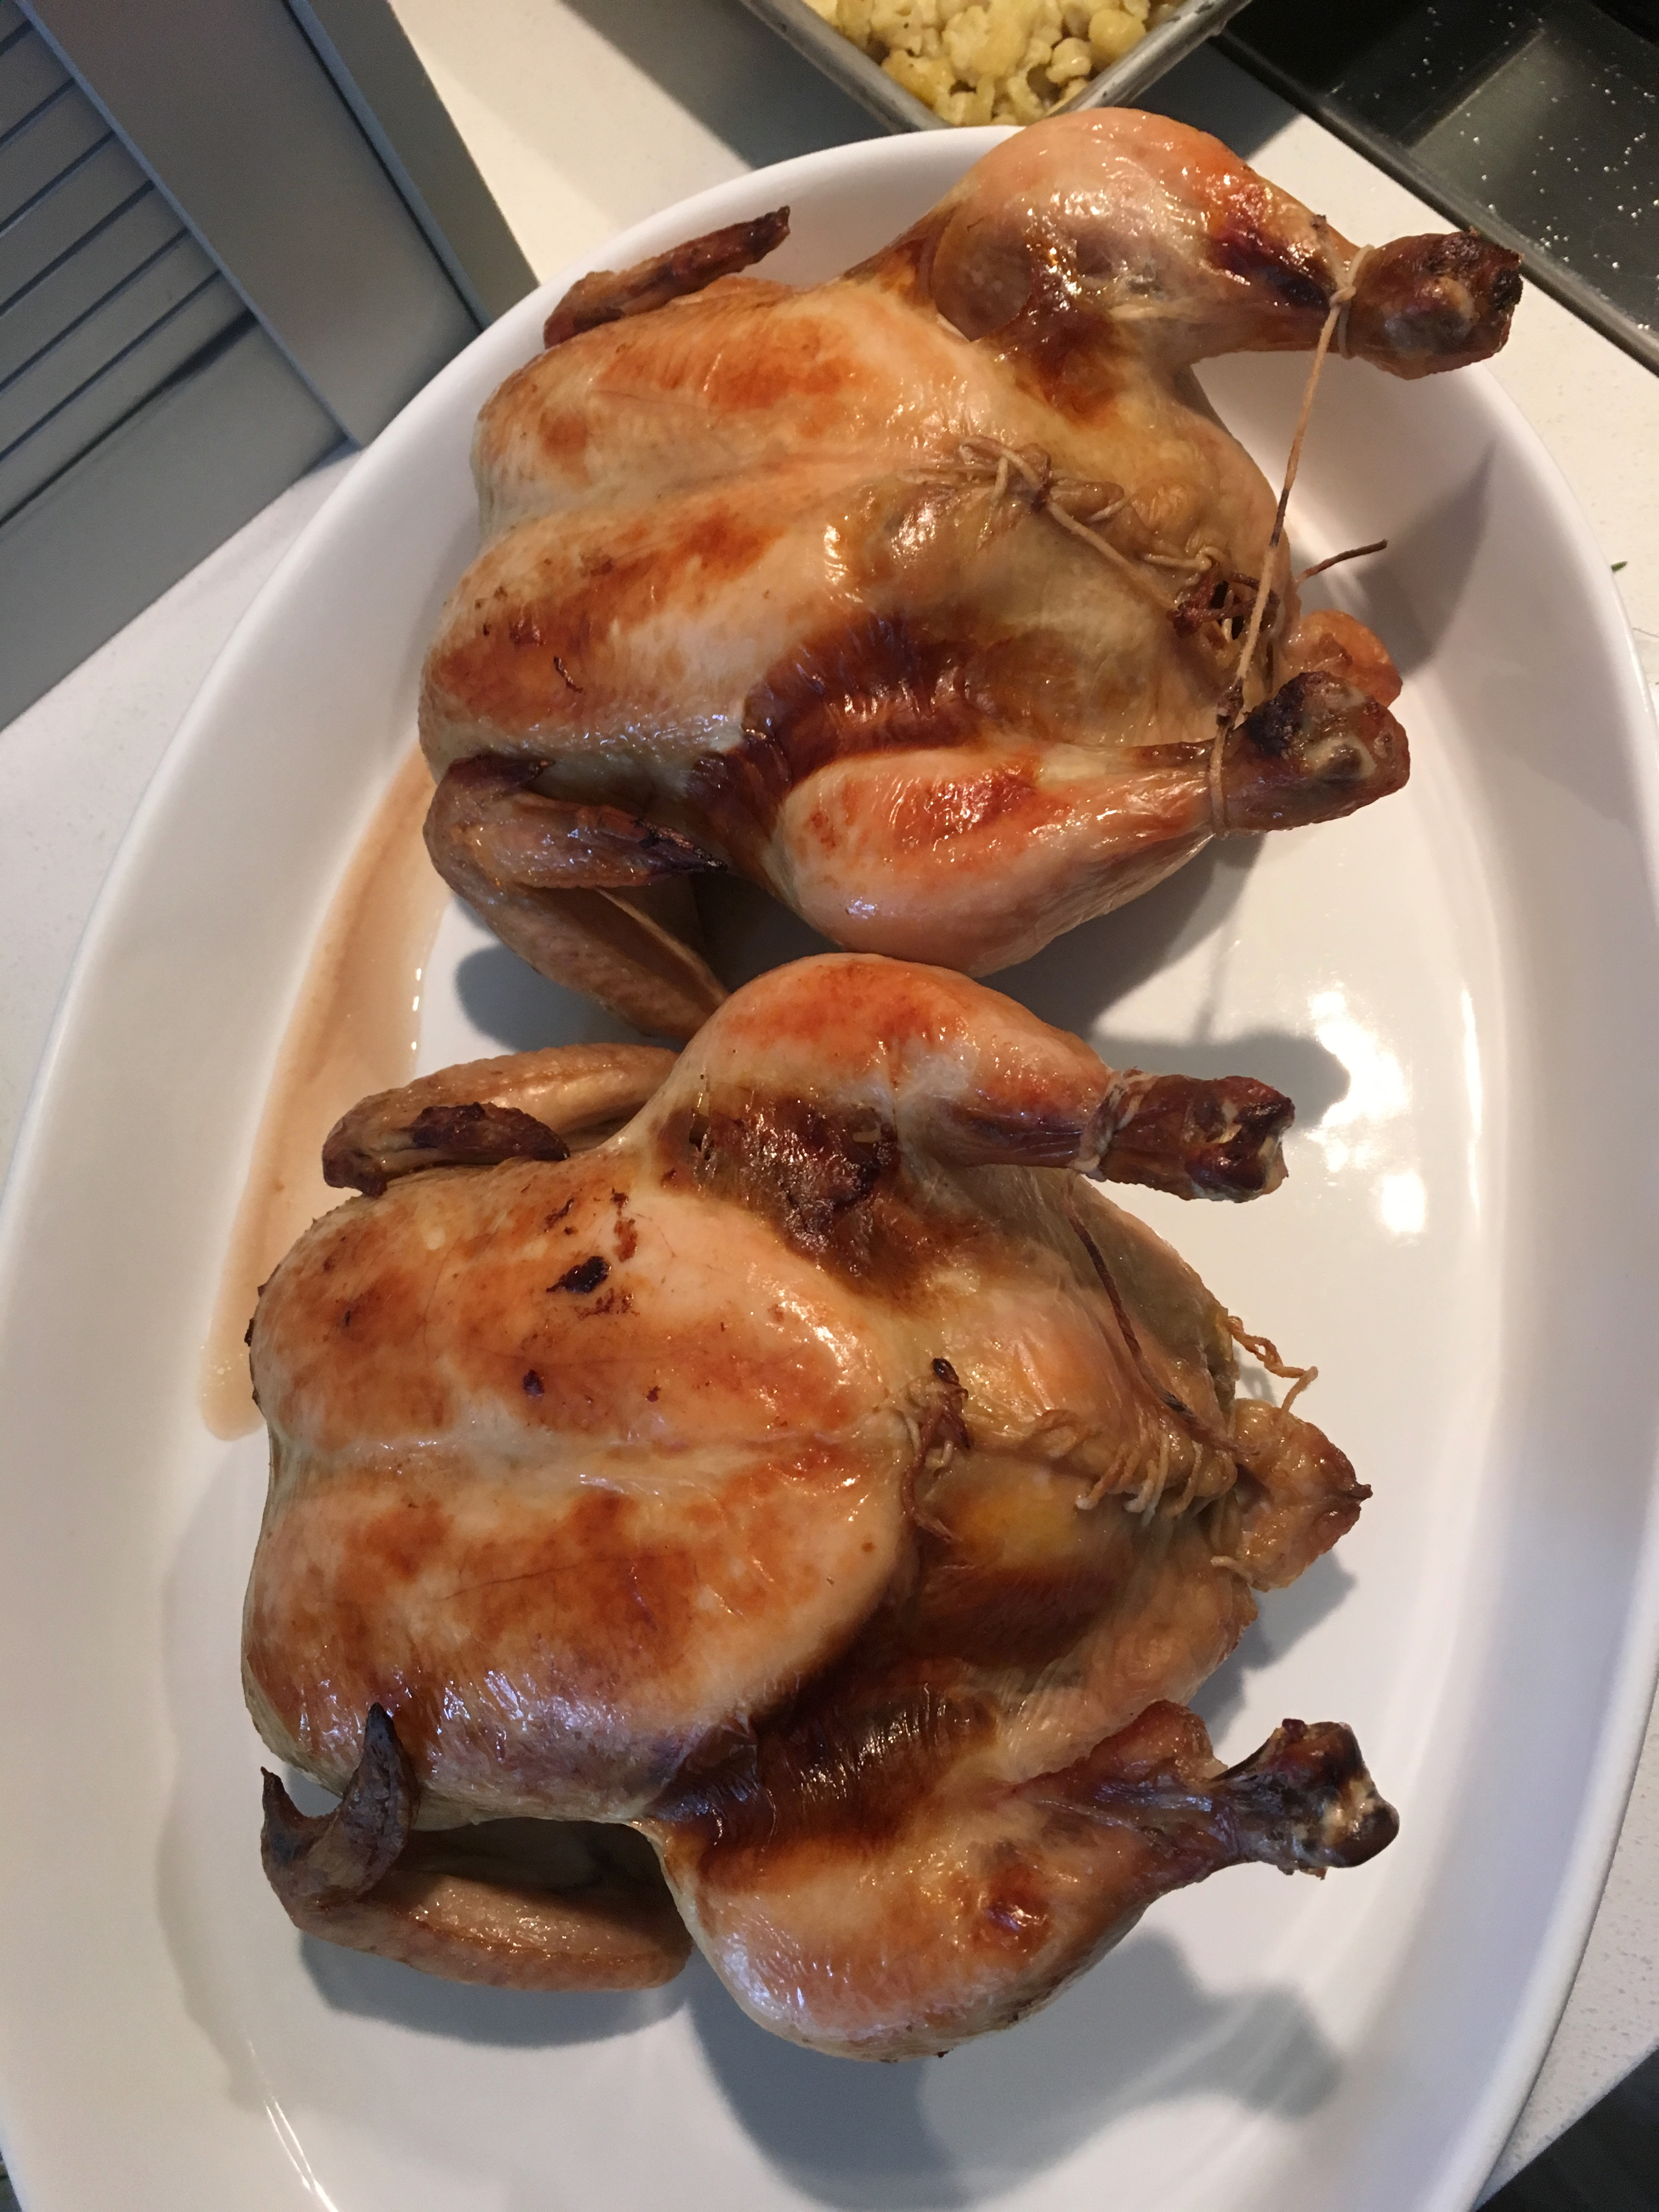
\includegraphics[width=0.25\textwidth]{\imageDir/\fileName/IMG_3228.jpg} \\
\end{tabular}
\end{table}


\end{document}




